\documentclass[12pt]{article}
\usepackage[utf8]{inputenc}
\usepackage[all]{xy}
\usepackage{bigfoot}
\usepackage{hyperref}
\usepackage{graphicx}
\usepackage{verbatim}
\usepackage{xcolor}
\usepackage{minted}
\usepackage{amsthm}
\graphicspath{ {images/} }

\theoremstyle{definition}
\newtheorem{theorem}{Teorema}[section]
\newtheorem{definition}{Definizione}[section]
\newtheorem{example}{Esempio}[section]
\newtheorem{exercise}{Esercizio}[section]
\newtheorem{observation}{Osservazione}[section]
\newtheorem{combinator}{Combinatore}[section]
\newtheorem{function}{Funzione}[section]

\newenvironment{demo}
    {\begin{center}
    \begin{tabular}{|p{0.9\textwidth}|}
    \hline\\
    }
    {
    \\\\\hline
    \end{tabular}
    \end{center}
    }

%\newenvironment{code}
%  {\verbatim}
%  {\endverbatim}

\definecolor{LightGray}{rgb}{0.98,0.98,0.98}
\newminted{typescript}{fontfamily=tt,bgcolor=LightGray}

\newenvironment{code}
  {\vspace{0.5cm} \VerbatimEnvironment\begin{typescriptcode}}
  {\end{typescriptcode} \vspace{0.2cm}}

\title{
  %\textit{A beautiful bind} \\
  % \textit{Monad Lisa} \\
  Introduzione alla programmazione funzionale
}
\author{Giulio Canti}

\begin{document}

\maketitle

\tableofcontents

\newpage

\section{Che cos'è la programmazione funzionale}

\begin{quote}
Though programming was born in mathematics, it has since largely been divorced from it.
The idea is that there's some higher level than the code in which you need to be able to think precisely,
and that mathematics actually allows you to think precisely about it - Leslie Lamport
\end{quote}

La programmazione funzionale usa \emph{modelli} formali per descrivere e meglio governare le \emph{implementazioni}.
E più l'implementazione si avvicina al suo corrispettivo ideale (il modello matematico)
più diventa facile ragionare sul sistema.

Ecco un parziale elenco di concetti sfruttati dalla programmazione funzionale

\begin{itemize}
  \item Higher-order functions (\texttt{map}, \texttt{reduce}, \texttt{filter},  \ldots)
  \item Funzioni pure
  \item Strutture dati immutabili
  \item Algebraic Data Types
  \item Trasparenza referenziale\footnote{An expression is said to be \emph{referentially transparent} if it can be replaced with its corresponding value without changing the program's behavior}
  \item Algebre (Semigruppi, Monoidi, \ldots)
  \item Teoria delle Categorie (Funtori, Funtori applicativi, Monadi, \ldots)
  \item Ottica funzionale
\end{itemize}

Nella programmazione funzionale sono innanzitutto le proprietà del codice ad essere portate in primo piano.

\begin{example}
Perché \texttt{map} è "più funzionale" di un ciclo \texttt{for}?

\begin{code}
const xs = [1, 2, 3]
const double = n => n * 2

const ys = []
for (var i = 0; i < xs.length; i++) {
  ys.push(double(xs[i]))
}

const zs = xs.map(double)
\end{code}

\end{example}

Un ciclo \texttt{for} è più flessibile: posso modificare l'indice di partenza, la condizione di fine e il passo.
Ma questo vuol dire anche che ci sono più possibilità di introdurre bachi e non ho alcuna garanzia sul risultato.
Una \texttt{map} invece mi da delle garanzie: gli elementi dell'input verrano processati tutti dal primo all'ultimo e
qualunque sia l'operazione che viene fatta nella callback, il risultato sarà sempre un array con lo stesso numero di elementi
dell'array di input.

\subsection{Quali sono i suoi obiettivi?}

\begin{itemize}
  \item Design pattern derivati dai modelli formali
  \item Programmazione modulare\footnote{By modular programming I mean the process of building large programs by gluing together smaller programs - Simon Peyton Jones}
  \item Gestire gli effetti in modo che valga la trasparenza referenziale
  \item Rendere gli stati illegali non rappresentabili
\end{itemize}

Vedremo come lo studio delle algebre e delle monadi permettano di raggiungere questi obiettivi in modo generale.

Il pattern fondamentale della programmazione funzionale è la \emph{componibilità}, ovvero la costruzione di piccole unità
che fanno qualcosa di specifico in grado di essere combinate al fine di ottenere entità più grandi e complesse.

\begin{demo}
\begin{center}
\textbf{DEMO}

\texttt{combinator.ts}
\end{center}
\end{demo}

Una gran parte delle tecniche utilizzate nella programmazione funzionale sono mutuate dalla matematica.

Facciamo due esempi che ci saranno utili anche in seguito

\begin{itemize}
  \item come catturare il concetto di computazione parallelizzabile?
  \item che cos'è una funzione pura?
\end{itemize}

\subsection{Un esempio di matematica applicata: la proprietà associativa}

Il concetto di computazione parallelizzabile (e distribuibile) può essere catturato dalla nozione di operazione associativa.

\begin{definition}
Sia $A$ un insieme, una operazione $*: A \times A \rightarrow A$ si dice \emph{associativa} se per ogni $a, b, c \in A$ vale

$$
(a * b) * c = a * ( b * c )
$$
\end{definition}

In altre parole la proprietà associativa garantisce che non importa l'ordine in cui vengono fatte le operazioni, il risultato sarà sempre lo stesso.

Possiamo quindi eliminare le parentesi, senza pericolo di ambiguità

$$
a * b * c
$$

\begin{example}
La concatenazione di stringhe gode della proprietà associativa.

\begin{code}
("a" + "b") + "c" = "a" + ("b" + "c") = "abc"
\end{code}
\end{example}

Se sappiamo che una data operazione gode della proprietà associativa possiamo suddividere una computazione in due sotto computazioni, ognuna delle quali può essere ulteriormente suddivisa

$$
a * b * c * d * e * f * g * h = \Big( ( a * b ) * ( c * d ) \Big) * \Big( ( e * f ) * ( g * h ) \Big)
$$

Le sotto computazioni possono essere distribuite ed eseguite parallelamente.

\subsection{Funzioni pure}

\begin{quote}
Una funzione pura è una procedura che dato lo stesso input restituisce sempre lo stesso output e non ha alcun side effect osservabile.
\end{quote}

Un tale enunciato informale può lasciare spazio a qualche dubbio

\begin{itemize}
\item che cos'è un "side effect"?
\item cosa vuol dire "osservabile"?
\item ma soprattutto, cosa si intende con "stesso"?
\end{itemize}

Vediamo una definizione formale del concetto di funzione

\begin{definition}
Una \emph{funzione} $f: X \rightarrow Y$ è un sottoinsieme $f$ di $X \times Y$ (il \emph{prodotto cartesiano} di $X$ e $Y$) tale che
per ogni $x \in X$ esiste esattamente un $y \in Y$ tale che $(x, y) \in f$\footnote{Questa definizione risale ad un secolo fa https://en.wikipedia.org/wiki/History\_of\_the\_function\_concept}.
\end{definition}

L'insieme $X$ si dice il \emph{dominio} di $f$, $Y$ il suo \emph{codominio}.

\begin{example}
La funzione $\texttt{double}: Nat \rightarrow Nat$ è il sottoinsieme del prodotto cartesiano $Nat \times Nat$ dato da $\{ (1, 2), (2, 4), (3, 6), \ldots \}$.
\end{example}

In TypeScript

\begin{code}
const f: { [key: number]: number } = {
  1: 2,
  2: 4,
  3: 6
  ...
}
\end{code}

Si noti che l'insieme $f$ deve essere descritto \emph{staticamente} in fase di definizione della funzione
(ovvero gli elementi di quell'insieme non possono variare nel tempo e per nessuna condizione interna o esterna).
Ecco allora che viene esclusa ogni forma di side effect e il risultato è sempre quello atteso.

Quella dell'esempio viene detta definizione \emph{estensionale} di una funzione, ovvero si enumerano uno per uno gli elementi dell'insieme.
Naturalmente quando l'insieme è infinito come in questo caso, la definizione può risultare un po' scomoda.

Si può ovviare a questo problema introducendo quella che viene detta definizione \emph{intensionale},
ovvero si esprime una condizione che deve valere per tutte le coppie $(x, y) \in f$ ovvero $y = x * 2$. Questa è la familiare forma con cui scriviamo la funzione $double$ e come la definiamo in JavaScript

\begin{code}
const double = x => x * 2
\end{code}

o in TypeScript, ove risultano evidenti dominio e codominio sottoforma di type annotation

\begin{code}
const double = (x: number): number => x * 2
\end{code}

La definizione di funzione come sottoinsieme di un prodotto cartesiano mostra come in matematica tutte le funzioni siano pure:
non c'è azione, modifica di stato o modifica degli elementi (che sono considerati immutabili) degli insiemi coinvolti.
Nella programmazione funzionale l'implementazione delle funzioni deve avvicinarsi il più possibile a questo modello ideale.

Che una funzione sia pura non implica necessariamente che sia bandita la mutabilità, localmente è ammissibile
se non esce dai confini della implementazione.

\begin{verbatim}
              Mutable
                 ^
      (Good)     |      (Bad)
                 |
  Non-Shared ----------> Shared
    State        |       State
                 |
      (Good)     |      (Good)
             Immutable
\end{verbatim}

Lo scopo ultimo è garantirne le proprietà fondamentali: purezza e trasparenza referenziale.

Infine le funzioni compongono

\begin{definition}
Siano $f: Y \rightarrow Z$ e $g: X \rightarrow Y$ due funzioni, allora la funzione $h: X \rightarrow Z$ definita da

$$
h(x) = f(g(x))
$$

si dice \emph{composizione} di $f$ e $g$ e si scrive $h = f \circ g$

\end{definition}

Si noti che affinchè due funzioni $f$ e $g$ possano comporre, il codominio di $g$ deve coincidere col dominio di $f$.

\subsection{Funzioni parziali}

\begin{definition}
Una funzione \emph{parziale} è una funzione che non è definita per tutti i valori del dominio.
\end{definition}

Viceversa una funzione definita per tutti i valori del dominio è detta \emph{totale}.

\begin{example}
$$
f(x) = \frac{1}{x}
$$
\end{example}

La funzione $f: number \rightarrow number$ non è definita per $x = 0$.

Una funzione parziale $f: X \rightarrow Y$ può essere sempre ricondotta ad una funzione totale aggiungendo un valore speciale,
chiamiamolo $None$, al codominio e associandolo ad ogni valore di $X$ per cui $f$ non è definita

$$
f': X \rightarrow Y \cup None
$$

Chiamiamo $Option(Y) = Y \cup None$.

$$
f': X \rightarrow Option(Y)
$$

In ambito funzionale si tende a definire solo funzioni totali.

\newpage

\section{Error handling funzionale}

Consideriamo la funzione

\begin{code}
const inverse = (x: number): number => 1 / x
\end{code}

Tale funzione è parziale perché non è definita per $x = 0$. Come possiamo gestire questa situazione?

Una soluzione potrebbe essere lanciare un'eccezione

\begin{code}
const inverse = (x: number): number => {
  if (x !== 0) return 1 / x
  throw new Error('cannot divide by zero')
}
\end{code}

ma così la funzione non sarebbe più da considerarsi pura
\footnote{Le eccezioni sono considerate un side effect inaccettabile perché modificano la normale esecuzione del codice
e violano la trasparenza referenziale}.

Un'altra possibile soluzione è restituire \texttt{null}

\begin{code}
const inverse = (x: number): number | null => {
  if (x !== 0) return 1 / x
  return null
}
\end{code}

Sorge però un nuovo problema quando si cerca di comporre la funzione \texttt{inverse} così modificata con un'altra funzione

\begin{code}
// calcola l'inverso e poi moltiplica per 2
const doubleInverse = (x: number): number => double(inverse(x))
\end{code}

L'implementazione di \texttt{doubleInverse} non è corretta, cosa succede se \texttt{inverse(x)} restituisce \texttt{null}?
Occorre tenerne conto

\begin{code}
const doubleInverse = (x: number): number | null => {
  const y = inverse(x)
  if (y === null) return null
  return double(y)
}
\end{code}

Appare evidente come l'obbligo di gestione del valore speciale \texttt{null} si propaghi in modo contagioso
a tutti gli utilizzatori di \texttt{inverse}.

Questo approccio ha diversi svantaggi

\begin{itemize}
  \item molto boilerplate
  \item prono ad errori (è facile dimenticarsi di gestire il caso di fallimento)
  \item le funzioni non compongono facilmente
\end{itemize}

\subsection{Il tipo \texttt{Option}}

La soluzione funzionale ai problemi illustrati precedentemente è l'utilizzo del tipo \texttt{Option},
eccone la definizione

\begin{code}
type Option<A> = None | Some<A>

class None {
  readonly _tag = 'None'
}

class Some<A> {
  readonly _tag = 'Some'
  constructor(readonly value: A) {}
}

// in TypeScript never è un bottom type
// ovvero un sottotipo di ogni altro tipo
const none: Option<never> = new None()

const some = <A>(a: A): Option<A> => new Some(a)
\end{code}

Ridefiniamo \texttt{inverse} sfruttando \texttt{Option}

\begin{code}
const inverse = (x: number): Option<number> =>
  x === 0 ? none : some(1 / x)
\end{code}

Possiamo interpretare questa modifica in termini di successo e fallimento: se viene restituita una istanza di \texttt{Some}
la computazione di \texttt{inverse} ha avuto successo, se viene restituita una istanza di \texttt{None} essa è fallita.

\begin{demo}
Il tipo \texttt{Option} codifica l'\emph{effetto} di una computazione che può fallire
\end{demo}

Aggiungiamo un metodo \texttt{map}

\begin{code}
type Option<A> = None<A> | Some<A>

class None<A> {
  readonly _tag = 'None'
  map<B>(f: (a: A) => B): Option<B> {
    return none
  }
}

class Some<A> {
  readonly _tag = 'Some'
  constructor(readonly value: A) {}
  map<B>(f: (a: A) => B): Option<B> {
    return some(f(this.value))
  }
}
\end{code}

In un linguaggio che non supporta classi e metodi, \texttt{map} può essere definita come funzione

\begin{code}
const map = <A, B>(
  f: (a: A) => B,
  fa: Option<A>
): Option<B> => {
  switch (fa._tag) {
    case 'None':
      return none
    case 'Some':
      return some(f(fa.value))
  }
}
\end{code}


Ora è possibile definire \texttt{doubleInverse} senza boilerplate

\begin{code}
const doubleInverse = (x: number): Option<number> =>
  inverse(x).map(double)

doubleInverse(2) // Some(1)
doubleInverse(0) // None
\end{code}

\begin{example}
Inoltre è facile concatenare altre operazioni

\begin{code}
const inc = (x: number): number => x + 1

inverse(0)
  .map(double)
  .map(inc) // None
inverse(4)
  .map(double)
  .map(inc) // Some(1.5)
\end{code}
\end{example}

\begin{demo}
\texttt{Option} mi permette di concentrarmi solo sul \emph{path di successo} in una serie di computazioni che possono fallire
\end{demo}

Per questioni di interoperabilità con codice che non usa \texttt{Option} possiamo definire due utili funzioni

\begin{code}
const fromNullable = <A>(
  a: A | null | undefined
): Option<A> => (a == null ? none : some(a))

const toNullable = <A>(fa: Option<A>): A | null => {
  switch (fa._tag) {
    case 'None':
      return null
    case 'Some':
      return fa.value
  }
}
\end{code}

\subsection{Branching tramite la funzione \texttt{fold}}

Prima o poi dovrò affrontare il problema di stabilire cosa fare sia nel caso di successo che di fallimento.
La funzione \texttt{fold} permette di gestire i due casi

\begin{code}
class Some<A> {
  ...
  fold<R>(f: () => R, g: (a: A) => R): R {
    return g(this.value)
  }
}

class None<A> {
  ...
  fold<R>(f: () => R, g: (a: A) => R): R {
    return f()
  }
}

const f = (): string => "cannot divide by zero"
const g = (x: number): string => "the result is " + x

inverse(2).fold(f, g) // 'the result is 0.5'
inverse(0).fold(f, g) // 'cannot divide by zero'
\end{code}

Si noti come il branching è racchiuso nella definizione di \texttt{Option} e non necessita di alcun \texttt{if}
e che l'utilizzo necessita solo di funzioni.

Inoltre le funzioni \texttt{f} e \texttt{g} sono generiche e riutilizzabili.

\subsection{Il tipo \texttt{Either}}

Il tipo \texttt{Option} è utile quando c'è un solo modo evidente per il quale una computazione può fallire,
oppure ce ne sono diversi ma non interessa distinguerli.

Se invece esistono molteplici ragioni di fallimento ed interessa comunicare al chiamante quale si sia verificata,
oppure se si vuole definire un errore personalizzato, è possibile impiegare il tipo \texttt{Either}. Eccone la definizione

\begin{code}
type Either<L, A> = Left<L, A> | Right<L, A>

class Left<L, A> {
  readonly _tag = 'Left'
  constructor(readonly value: L) {}
  map<B>(f: (a: A) => B): Either<L, B> {
    return left(this.value)
  }
}

class Right<L, A> {
  readonly _tag = 'Right'
  constructor(readonly value: A) {}
  map<B>(f: (a: A) => B): Either<L, B> {
    return right(f(this.value))
  }
}

const left = <L, A>(l: L): Either<L, A> =>
  new Left(l)

const right = <L, A>(a: A): Either<L, A> =>
  new Right(a)
\end{code}

Tipicamente \texttt{Left} rappresenta il caso di fallimento mentre \texttt{Right} quello di successo.

Ridefiniamo la funzione \texttt{inverse} in funzione del tipo \texttt{Either}

\begin{code}
const inverse = (x: number): Either<string, number> =>
  x === 0 ? left('cannot divide by zero') : right(1 / x)
\end{code}

Ancora una volta è possibile definire \texttt{doubleInverse} senza boilerplate

\begin{code}
const doubleInverse = (x: number): Either<string, number> =>
  inverse(x).map(double)

doubleInverse(2) // Right(1)
doubleInverse(0) // Left('cannot divide by zero')
\end{code}

ed è facile comporre insieme altre operazioni

\begin{code}
inverse(0)
  .map(double)
  .map(inc) // Left('cannot divide by zero')
inverse(4)
  .map(double)
  .map(inc) // Right(1.5)
\end{code}

Anche per il tipo \texttt{Either} è possibile definire una funzione \texttt{fold}

\begin{code}
class Left<L, A> {
  ...
  fold<R>(f: (l: L) => R, g: (a: A) => R): R {
    return f(this.value)
  }
}

class Right<L, A> {
  ...
  fold<R>(f: (l: L) => R, g: (a: A) => R): R {
    return g(this.value)
  }
}
\end{code}

I vantaggi offerti dalla funzione \texttt{map} non sono esclusivi dei tipi \texttt{Option} e \texttt{Either}.
Essi sono condivisi da tutti i membri di una vasta famiglia che prende il nome di \emph{funtori}. Per definire in modo formale cosa sia un funtore,
occorre prima introdurre il concetto di \emph{categoria}.

\section{Teoria delle categorie}

\subsection{Perché è importante?}

\begin{quote}
And how do we solve problems? We decompose bigger problems into smaller problems. If the smaller problems are still too big,
we decompose them further, and so on. Finally, we write code that solves all the small problems.
And then comes the essence of programming: we compose those pieces of code to create solutions to larger problems.
Decomposition wouldn’t make sense if we weren’t able to put the pieces back together. - Bartosz Milewski
\end{quote}

Ma cosa vuol dire esattamente \emph{componibile}? Quando possiamo davvero dire che due cose \emph{compongono}?
E se compongono quando possiamo dire che lo fanno in un \emph{modo buono}?\\

\begin{quote}
Entities are composable if we can easily and generally combine their behaviors in some way without having to modify the entities being combined.
I think of composability as being the key ingredient necessary for acheiving reuse, and for achieving a combinatorial expansion of
what is succinctly expressible in a programming model. - Paul Chiusano
\end{quote}

Occorre poter fare riferimento ad una teoria \textbf{rigorosa} che possa fornire risposte a domande così fondamentali.

Opportunamente da più di 60 anni un vasto gruppo di studiosi appartenenti al più longevo e mastodontico progetto open source nella storia
dell'umanità si occupa di sviluppare una teoria specificatamente dedicata a questo argomento: la \emph{componibilità}.

Il progetto open source si chiama \emph{matematica} e la teoria sulla componibilità ha preso il nome di \emph{Teoria delle categorie}.

Studiare teoria delle categorie non è perciò un passatempo astratto, ma va dritto al cuore di ciò che facciamo tutti i giorni quando vogliamo
sviluppare (buon) software.

\subsection{Definizione}

\begin{definition}
Una \emph{categoria} $\mathcal{C}$ è una coppia $(O, M)$ ove

\begin{itemize}
  \item $O$ è una collezione di \emph{oggetti}, non meglio specificati. Considerate un oggetto come un corpo imperscrutabile,
  senza struttura né proprietà distintive, a meno della sua identità (ovvero considerati due oggetti sappiamo solo se sono uguali oppure diversi
  ma non il perché).
  \item $M$ è una collezione di \emph{frecce} (o \emph{morfismi}) che collegano gli oggetti. Tipicamente un morfismo $f$ è denotato con $f: A \rightarrow B$
  per rendere chiaro che è una freccia che parte da $A$ detta \emph{sorgente} e arriva a $B$ detta \emph{destinazione}.
\end{itemize}

Mentre gli oggetti non hanno ulteriori proprietà da soddisfare, per i morfismi devono valere alcune condizioni note come \emph{leggi}\\

\paragraph{Morfismi identità.} Per ogni oggetto $X$ di $\mathcal{C}$ deve esistere un morfismo $1_X: X \rightarrow X$ (chiamato \emph{morfismo identità per $X$})\\

\paragraph{Composizione di morfismi.} Deve esistere una operazione, indichiamola con il simbolo $\circ$, detta \emph{composizione}, tale che per ogni coppia di morfismi $g: A \rightarrow B$
e $f: B \rightarrow C$ associa un terzo morfismo $f \circ g: A \rightarrow C$. Inoltre l'operazione $\circ$ di composizione deve soddisfare le seguenti proprietà:

\begin{itemize}
  \item associatività: se $g: A \rightarrow B$, $f: B \rightarrow C$, $h: C \rightarrow D$, allora $h \circ (f \circ g) = (h \circ f) \circ g$
  \item identità: per ogni morfismo $f: A \rightarrow B$ vale $f \circ 1_A = f = 1_B \circ f$ (ove $1_A$ e $1_B$ sono rispettivamente i morfismi identità di $A$ e $B$)
\end{itemize}

\end{definition}

\begin{example}
\[
\xymatrixrowsep{3cm}
\xymatrixcolsep{3cm}
\xymatrix{
  A \ar@(ul,ur)^{1_A} \ar[r]^g \ar[rd]_{f \circ g} & B \ar@(ul,ur)^{1_B} \ar[d]^f \\
    & C \ar@(dl,dr)_{1_C}
}
\]
\end{example}

\subsection{Linguaggi di programmazione come categorie}

Un linguaggio di programmazione può essere modellato da una categoria ove

\begin{itemize}
\item i tipi sono gli oggetti
\item le funzioni sono i morfismi
\item l'operazione di composizione è la composizione di funzioni
\end{itemize}

\begin{example}
Un semplice linguaggio di programmazione con tre tipi e tre funzioni

\[
\xymatrixrowsep{3cm}
\xymatrixcolsep{3cm}
\xymatrix{
  {\texttt{string}} \ar[r]^{length} \ar[rd]_{length > 2} & {\texttt{number}} \ar[d]^{> 2} \\
    & {\texttt{boolean}}
}
\]
\end{example}

\begin{code}
const length = (s: string): number => s.length

const gt2 = (n: number): boolean => n > 2

const lengthGt2 = compose(gt2, length)
\end{code}

\newpage

\section{Funtori}

Di fronte ad un nuovo oggetto di studio come le categorie, il matematico ha davanti due percorsi di indagine: il primo, che chiamerò, \emph{ricerca in profondità},
mira a studiare le proprietà di una singola categoria. Il secondo (ed è quello che interessa a noi), che chiamerò \emph{ricerca in ampiezza},
mira a studiare quando due categorie possono essere dette \emph{simili}.

Per iniziare questo secondo tipo di indagine dobbiamo introdurre un nuovo strumento: le mappe tra categorie
(pensate a mappa come ad un sinonimo di funzione).

\paragraph{Mappe tra categorie.} Se $\mathcal{C}$ e $\mathcal{D}$ sono due categorie, cosa vuol dire costruire una mappa $F$ tra $\mathcal{C}$ e $\mathcal{D}$?

Essenzialmente vuol dire costruire una associazione tra le parti costituenti di $\mathcal{C}$ e le parti costituenti di $\mathcal{D}$.

Siccome una categoria è composta da due cose, i suoi oggetti e i suoi morfismi, per avere una buona mappa non devo mischiarle,
devo cioè fare in modo che agli oggetti di $\mathcal{C}$ vengano associati degli oggetti di $\mathcal{D}$ e che ai morfismi di
$\mathcal{C}$ vengano associati dei morfismi di $\mathcal{D}$.

La costruzione di una buona mappa implica che oggetti e morfismi viaggiano su strade separate e non si mischiano tra loro.

Ma mi interessano proprio tutte le mappe che posso costruire così? No davvero, molte di quelle che posso costruire
non sarebbero affatto interessanti: quello che voglio è perlomeno preservare la \emph{struttura di categoria},
ovvero che le leggi rimangano valide anche dopo aver applicato la mappa.

Specifichiamo in modo formale che cosa vuol dire per una mappa preservare la struttura categoriale.

\subsection{Definizione}

\begin{definition}
Siano $\mathcal{C}$ e $\mathcal{D}$ due categorie, allora una mappa $F$ si dice \emph{funtore} se valgono le seguenti proprietà:

\begin{itemize}
  \item ad ogni oggetto $X$ in $\mathcal{C}$, $F$ associa un oggetto $F(X)$ in $\mathcal{D}$
  \item ad ogni morfismo $f: A \rightarrow B$ in $\mathcal{C}$, $F$ associa un morfismo $F(f): F(A) \rightarrow F(B)$ in $\mathcal{D}$
  \item $F(1_X) = 1_{F(X)}$ per ogni oggetto $X$ in $\mathcal{C}$
  \item $F(f \circ_\mathcal{C} g) = F(f) \circ_\mathcal{D} F(g)$ per tutti i morfismi $g: A \rightarrow B$ e $f: B \rightarrow C$ in $\mathcal{C}$
\end{itemize}

\end{definition}

Le prime due proprietà formalizzano il requisito che oggetti e morfismi viaggiano su strade separate.

Le ultime due formalizzano il requisito che la struttura categoriale sia preservata.

\begin{observation}
L'ultima legge permette delle ottimizzazioni, passando da

\begin{code}
inverse(4)
  .map(double)
  .map(inc)
\end{code}

a

\begin{code}
inverse(4)
  .map(compose(inc, double))
\end{code}
\end{observation}

\subsection{Diagramma dell'azione di un funtore}

\[
\xymatrixrowsep{3cm}
\xymatrixcolsep{3cm}
\xymatrix{
  F(A) \ar[r]^{F(g)} \ar[r] \ar@/^1cm/[rr]^{F(f) \circ_\mathcal{D} F(g)} & F(B) \ar[r]^{F(f)} & F(C) \ar@(ul,ur)^{F(1_C)} & \mathcal{D} \\
  A \ar[u]^F \ar[r]_g \ar@/_1cm/[rr]_{f \circ_\mathcal{C} g}  & B \ar[u]^F \ar[r]_f & C \ar[u]^F \ar@(dl,dr)_{1_C} & \mathcal{C}
}
\]

L'associazione tra $f$ e $F(f)$ si chiama \emph{lifting} del morfismo $f$.

Quando $\mathcal{C}$ e $\mathcal{D}$ coincidono, si parla di \emph{endofuntori} \footnote{endo proviene dal greco e significa dentro}.

\begin{exercise}
Mostrare che $F(\mathcal{C})$ è una sotto-categoria di $\mathcal{D}$.
\end{exercise}

\subsection{La categoria $\mathcal{TS}$}

Vediamo la categoria che rappresenta il linguaggio \texttt{TypeScript}, come ogni categoria,
la categoria $\mathcal{TS}$ è composta da oggetti e morfismi

\begin{itemize}
  \item gli oggetti sono i tipi (per esempio \texttt{number}, \texttt{string}, \texttt{boolean}, \texttt{Array<number>}, \texttt{Array<Array<number>>}, etc \ldots)
  \item i morfismi sono funzioni tra tipi (per esempio \texttt{number $\rightarrow$ number}, \texttt{string $\rightarrow$ number}, \texttt{Array<number> $\rightarrow$ Array<number>}, etc \ldots)
  \item l'operazione di composizione $\circ$ è l'usuale composizione di funzioni.
\end{itemize}

\subsection{Endofuntori in $\mathcal{TS}$}

Definire un (endo)funtore $F$ nella categoria $\mathcal{TS}$ significa due cose:

\begin{itemize}
  \item per ogni tipo $A$ stabilire a quale tipo corrisponde $F(A)$
  \item per ogni funzione $f: A \rightarrow B$ stabilire a quale funzione corrisponde $F(f)$
\end{itemize}

Perciò un funtore è una coppia $F = (\texttt{F<X>}, \texttt{lift})$ ove

\begin{itemize}
  \item \texttt{F} è un \emph{type constructor}\footnote{
    ovvero una procedura che, dato un qualunque tipo \texttt{X} produce un tipo \texttt{F<X>} come per esempio \texttt{Option} o \texttt{Array}
    \begin{itemize}
      \item \texttt{number} è un $0$-type constructor (kind $*$)
      \item \texttt{Option<A>} è un $1$-type constructor (kind $* \rightarrow *$)
      \item \texttt{Either<L, A>} è un $2$-type constructor (kind $* \rightarrow * \rightarrow *$)
    \end{itemize}
  }
  \item \texttt{lift} è una funzione con la seguente firma
\end{itemize}

\begin{code}
lift: <A, B>(f: (a: A) => B) => (fa: F<A>) => F<B>
\end{code}

La funzione \texttt{lift} è meglio conosciuta nella sua forma equivalente \texttt{map}.

\begin{code}
map: <A, B>(f: (a: A) => B, fa: F<A>) => F<B>
\end{code}

Possiamo rappresentare il concetto di funtore mediante una interfaccia

\begin{code}
interface Functor<F> {
  map: <A, B>(f: (a: A) => B, fa: F<A>) => F<B>
}
\end{code}

Vediamo l'implementazione per \texttt{Option} e \texttt{Either}

\begin{code}
// Option
const funtorOption = {
  map: <A, B>(f: (a: A) => B, fa: Option<A>): Option<B> =>
    fa.fold(() => none, a => some(f(a)))
}

// Either
const functorEither = {
  map: <L, A, B>(
    f: (a: A) => B,
    fa: Either<L, A>
  ): Either<L, B> => fa.fold(left, a => right(f(a)))
}
\end{code}

Per comodità di utilizzo (\emph{chainable APIs}) abbiamo già visto che è utile implementare \texttt{map} in modo che
l'argomento \texttt{fa} sia implicito (ovvero implementare \texttt{map} come metodo del type constructor \texttt{F})

\begin{code}
// Option
class None<A> {
  ...
  map<B>(f: (a: A) => B): Option<B> {
    return none
  }
}

class Some<A> {
  ...
  map<B>(f: (a: A) => B): Option<B> {
    return some(f(this.value))
  }
}

// Either
class Left<L, A> {
  ...
  map<B>(f: (a: A) => B): Either<L, B> {
    return left(this.value)
  }
}

class Right<L, A> {
  ...
  map<B>(f: (a: A) => B): Either<L, B> {
    return right(f(this.value))
  }
}
\end{code}

\subsection{Esempi}

Vediamo una raccolta dei funtori più comuni

\begin{example}
Il funtore \textbf{Identity} manda un tipo \texttt{A} ancora in \texttt{A}

\begin{code}
class Identity<A> {
  constructor(readonly value: A) {}
  map<B>(f: (a: A) => B): Identity<B> {
    return new Identity(f(this.value))
  }
}
\end{code}
\end{example}

\begin{example}
Il funtore \textbf{Array} manda un tipo \texttt{A} nel tipo della lista di elementi di tipo \texttt{A}

\begin{code}
const functorArray = {
  map: <A, B>(f: (a: A) => B, fa: Array<A>): Array<B> =>
    fa.map(f)
}
\end{code}
\end{example}

\begin{example}
Il funtore \textbf{IO} manda un tipo \texttt{A} nel tipo \texttt{() => A}\footnote{Una funzione senza argomenti viene detta \emph{thunk}}

\begin{code}
class IO<A> {
  constructor(readonly run: () => A) {}
  map<B>(f: (a: A) => B): IO<B> {
    return new IO(() => f(this.run()))
  }
}
\end{code}
\end{example}

\begin{example}
Il funtore \textbf{Task} manda un tipo \texttt{A} nel tipo \texttt{() => Promise<A>}.

Le \texttt{Promise} sono \emph{eager}, ovvero eseguono il side effect immediatamente, \texttt{Task} è una variante \emph{lazy}
di una computazione asincrona

\begin{code}
class Task<A> {
  constructor(readonly run: () => Promise<A>) {}
  map<B>(f: (a: A) => B): Task<B> {
    return new Task(() => this.run().then(f))
  }
}
\end{code}
\end{example}

\begin{exercise}
Sia

\begin{code}
type Tuple<L, A> = [L, A]
\end{code}

definire una istanza di funtore.
\end{exercise}

\begin{observation}
Non tutte le istanze di funtore sono associabili ad un "contenitore", come mostrato dall'esercizio seguente
\end{observation}

\begin{exercise}
Sia

\begin{code}
type Decoder<A> = (s: string) => A
\end{code}

definire una istanza di funtore.

Più in generale definire una istanza di funtore per il seguente tipo

\begin{code}
type Reader<E, A> = (e: E) => A
\end{code}

con \texttt{E} fissato

\end{exercise}

\subsection{Composizione di funtori}

I funtori compongono e la \texttt{map} della composizione è la composizione delle \texttt{map}.

Formalmente, siano $F: \mathcal{D} \rightarrow \mathcal{E}$ e $G: \mathcal{C} \rightarrow \mathcal{D}$ due funtori,
allora possiamo costruire il funtore composizione $F(G): \mathcal{C} \rightarrow \mathcal{E}$

\[
\xymatrixrowsep{3cm}
\xymatrixcolsep{3cm}
\xymatrix{
  F(G(A)) \ar[r]^{F(G(g))} \ar[r] & F(G(B)) \ar[r]^{F(G(f))} & F(G(C)) & \mathcal{E} \\
  G(A) \ar[u]^F \ar[r]^{G(g)} \ar[r] & G(B) \ar[u]^F \ar[r]^{G(f)} & G(C) \ar[u]^F & \mathcal{D} \\
  A \ar[u]^G \ar[r]_g & B \ar[u]^G \ar[r]_f & C \ar[u]^G & \mathcal{C}
}
\]

\begin{example}
Una istanza di funtore per gli array di \texttt{Option}

\begin{code}
class ArrayOption<A> {
  constructor(readonly value: Array<Option<A>>) {}
  map<B>(f: (a: A) => B): ArrayOption<B> {
    return new ArrayOption(this.value.map(o => o.map(f)))
  }
}
\end{code}
\end{example}

\newpage

\section{Funtori controvarianti}

\begin{code}
// Funtori covarianti
map: <A, B>      (f: (a: A) => B, fa: F<A>) => F<B>

// Funtori controvarianti
contramap: <A, B>(f: (b: B) => A, fa: F<A>) => F<B>
\end{code}

Come esempi di tipi che ammettono istanze di funtore controvariante consideriamo

\begin{itemize}
  \item i predicati\footnote{\texttt{type Predicate<A> = (a: A) => boolean}}
  \item le relazioni di equivalenza\footnote{\texttt{type Equivalence<A> = (x: A, y: A) => boolean}}
  \item le funzioni di ordinamento\footnote{\texttt{type Comparison<A> = (x: A, y: A) => -1 | 0 | 1}}
  \item i serializzatori\footnote{\texttt{type Encoder<A> = (a: A) => string}}
\end{itemize}

\begin{example}
Vediamo un esempio con i predicati

\begin{code}
type Predicate<A> = (a: A) => boolean

const contramap = <A, B>(
  f: (b: B) => A,
  predicate: Predicate<A>
): Predicate<B> => {
  return b => predicate(f(b))
}

const isAdult: Predicate<number> = age => age >= 18

interface Person {
  name: string
  age: number
}

const isPersonAdult: Predicate<Person> = contramap(
  p => p.age,
  isAdult
)

isPersonAdult({ name: 'Giulio', age: 45 }) // true
isPersonAdult({ name: 'Matilde', age: 2 }) // false
\end{code}
\end{example}

\begin{example}
Vediamo un altro esempio notevole di funtore controvariante: le componenti di \texttt{React}.

Il funtore \textbf{Component} manda un tipo \texttt{A} nel tipo

\begin{code}
(a: A) => ReactElement
\end{code}

\begin{code}
import * as React from 'react'
import * as ReactDOM from 'react-dom'

type Component<A> = (a: A) => React.ReactElement<any>

const contramap = <A, B>(
  f: (b: B) => A,
  component: Component<A>
): Component<B> => {
  return b => component(f(b))
}

const DisplayFullName = (a: { fullName: string }) => (
  <div>Hello {a.fullName}</div>
)

ReactDOM.render(
  <DisplayFullName fullName="Giulio Canti" />,
  document.getElementById('app')
)

type Person = {
  name: string
  surname: string
}

const DisplayPerson: Component<Person> = contramap(
  b => ({ fullName: `${b.name} ${b.surname}` }),
  DisplayFullName
)

ReactDOM.render(
  <DisplayPerson name="Giulio" surname="Canti" />,
  document.getElementById('app')
)
\end{code}
\end{example}

\newpage

\section{Bifuntori}

Un \emph{bifuntore} è un concetto associato ad un type constructor con kind \texttt{* -> * -> *}
per il quale esiste una istanza di funtore covariante per ambedue i type parameter.

La sua operazione è chiamata \texttt{bimap}

\begin{code}
interface Bifunctor<F> {
  bimap: <L, A, M, B>(
    fla: F<L, A>,
    f: (l: L) => M,
    g: (a: A) => B
  ) => F<M, B>
}
\end{code}

e deve valere la seguente identità

\begin{code}
bimap(x, identity, identity) = x
\end{code}

Vediamo un esempio, una istanza per \texttt{Either}

\begin{code}
const bimap = <L, V, A, B>(
  fla: Either<L, A>,
  f: (l: L) => V,
  g: (a: A) => B
): Either<V, B> => {
  return fla.fold(l => left(f(l)), a => right(g(a)))
}
\end{code}

\newpage

\section{Profuntori}

Vediamo ora un particolare type constructor che ammette sia una istanza di funtore covariante sia una istanza di
funtore controvariante: le funzioni.

\begin{code}
// I = input, O = output
type Function1<I, O> = (i: I) => O
\end{code}

Si noti che \texttt{Function1} ha kind \texttt{* -> * -> *} dato che
ha due type parameter \footnote{In Haskell \texttt{Function1} è indicato con \texttt{(->)}}.

Nel cercare una istanza di funtore abbiamo perciò due scelte

\begin{itemize}
\item fissare il type parameter \texttt{I}
\item fissare il type parameter \texttt{O}
\end{itemize}

Prima fissiamo il tipo in input \texttt{I} e otteniamo una istanza di funtore \textbf{covariante}

\begin{code}
const functorFunction1 = {
  map: <I, A, B>(
    f: (a: A) => B,
    fa: Function1<I, A>
  ): Function1<I, B> => {
    return i => f(fa(i))
  }
}
\end{code}

Notate che l'implementazione di \texttt{map} non è altro che la composizione di funzioni

\begin{code}
// prima g poi f
const compose = <I, A, B>(
  f: (a: A) => B,
  g: (i: I) => A
): ((i: I) => B) => {
  return i => f(g(i))
}

const functorFunction1 = {
  map: compose
}
\end{code}

Ora fissiamo il tipo in output \texttt{O} e otteniamo una istanza di funtore \textbf{controvariante}

\begin{code}
const contravariantFunction1 = {
  contramap: <B, A, O>(
    f: (b: B) => A,
    fa: Function1<A, O>
  ): Function1<B, O> => {
    return b => fa(f(b))
  }
}
\end{code}

Notate che l'implementazione di \texttt{contramap} non è altro che la funzione \texttt{pipe}

\begin{code}
// prima f poi g
const pipe = <B, A, O>(
  f: (b: B) => A,
  g: (a: A) => O
): ((b: B) => O) => {
  return b => g(f(b))
}

const contravariantFunction1 = {
  contramap: pipe
}
\end{code}

Giungiamo alla definizione di \texttt{Profunctor}, concetto associato ad un type constructor con kind \texttt{* -> * -> *} che è
controvariante nel primo type parameter e covariante nel secondo type parameter.

La sua operazione è chiamata \texttt{promap} (sinonimo \texttt{dimap})

\begin{code}
interface Profunctor<P> {
  promap: <A, B, C, D>(
    pbc: P<B, C>,
    f: (a: A) => B,
    g: (c: C) => D
  ) => P<A, D>
}
\end{code}

Tale che \texttt{promap(x, identity, identity) = x}

Alternativamente è possibile definire la coppia \texttt{lmap} e \texttt{rmap}.

\begin{code}
lmap: <A, B, C>(f: (a: A) => B, pbc: P<B, C>) => P<A, C>

rmap: <A, B, C>(f: (b: B) => C, pab: P<A, B>) => P<A, C>
\end{code}

Tali che \texttt{lmap(identity, x) = x} e \texttt{rmap(identity, x) = x}.

\begin{observation}
Deve valere la seguente relazione

\begin{code}
promap(f, g, x) = lmap(f, rmap(g, x))
\end{code}
\end{observation}

\newpage

\section{Semigruppi}

\subsection{Cos'è una algebra?}

Potremmo aggiungere al termine programmazione funzionale quello di programmazione algebrica, infatti

\begin{demo}
Le algebre sono i design pattern della programmazione funzionale
\end{demo}

Per algebra si intende generalmente una qualunque combinazione di

\begin{itemize}
  \item insiemi
  \item operazioni
  \item leggi
\end{itemize}

Le algebre sono il modo in cui i matematici tendono a catturare un concetto nel modo più puro,
ovvero eliminando tutto ciò che è superfluo.

Le algebre possono essere considerate una versione più potente delle interfacce: quando si manipola una struttura algebrica
sono permesse solo le operazioni definite dall'algebra in oggetto e in conformità alle sue leggi.

I matematici lavorano con tali interfacce da secoli e funziona in modo egregio.

Vediamo un esempio di algebra, il magma.

\subsection{Definizione di Magma}

\begin{definition}
Sia $M$ un insieme e $*$ un'operazione \emph{chiusa su} (o \emph{interna a}) $M$ ovvero $*: M \times M \rightarrow M$,
allora la coppia $(M, *)$ si chiama \emph{magma}.
\end{definition}

\begin{quote}
Because the binary operation of a magma takes two values of a given type and returns a new value of the same type (\emph{closure property}),
this operation can be chained indefinitely
\end{quote}

Il fatto che l'operazione sia chiusa è una proprietà non banale,
per esempio sui numeri naturali la somma è una operazione chiusa mentre la sottrazione non lo è.

Un magma non possiede alcuna legge a parte il vincolo basilare di chiusura, vediamo un'algebra che ne definisce una: i semigruppi.

\subsection{Definizione di Semigruppo}

\begin{definition}
Sia $(S, *)$ un magma, se $*$ è associativa \footnote{ovvero per ogni $a, b, c \in S$ vale

$$
(a * b) * c = a * ( b * c )
$$
} allora è un \emph{semigruppo}.
\end{definition}

L'insieme $S$ si dice insieme \emph{sostegno} del semigruppo.

La proprietà associativa ci assicura che non ci dobbiamo preoccupare di utilizzare le parentesi in una espressione\footnote{ovvero possiamo scrivere semplicemente $a * b * c$}.

Come abbiamo visto nell'introduzione, i semigruppi catturano l'essenza di una operazione parallelizzabile

Ma possono anche essere usati per rappresentare l'idea astratta di

\begin{itemize}
  \item concatenare
  \item fondere (merging)
  \item ridurre
  \item combinare
\end{itemize}

Vediamo qualche esempio

\begin{itemize}
  \item \texttt{(number, +)} ove \texttt{+} è l'usuale addizione di numeri
  \item \texttt{(number, *)} ove \texttt{*} è l'usuale moltiplicazione di numeri
  \item \texttt{(string, +)} ove \texttt{+} è l'usuale concatenazioni di stringhe
  \item \texttt{(boolean, \&\&)} ove \texttt{\&\&} è l'usuale congiunzione
  \item \texttt{(boolean, ||)} ove \texttt{||} è l'usuale disgiunzione
\end{itemize}

\subsection{Implementazione}

Come facciamo a tradurre questa astrazione sottoforma di codice?

Possiamo implementare il concetto di semigruppo come una \texttt{interface}

\begin{code}
interface Semigroup<A> {
  concat: (x: A, y: A) => A
}
\end{code}

L'insieme sostegno è rappresentato dal type parameter \texttt{A} mentre l'operazione $*$ è chiamata \texttt{concat}.

L'associatività non può essere espressa nel type system di TypeScript

\begin{code}
// deve valere per ogni a, b, c
concat(concat(a, b), c) = concat(a, concat(b, c))
\end{code}

Ecco come possiamo implementare il semigruppo $(number, +)$

\begin{code}
const sum: Semigroup<number> = {
  concat: (x, y) => x + y
}
\end{code}

Notate che si possono definire differenti istanze di semigruppo per lo stesso insieme sostegno

\begin{code}
const product: Semigroup<number> = {
  concat: (x, y) => x * y
}
\end{code}

\begin{exercise}
Implementare i seguenti semigruppi
\begin{itemize}
  \item \texttt{(string, +)}
  \item \texttt{(boolean, \&\&)}
  \item \texttt{(boolean, ||)}
  \item \texttt{(object, ...)} (spread operator)
\end{itemize}
\end{exercise}

L'insieme sostegno può essere costituito anche da funzioni

\begin{code}
type Predicate<A> = (a: A) => boolean

const getPredicateSemigroup = <A>(
  S: Semigroup<boolean>
): Semigroup<Predicate<A>> => ({
  concat: (x, y) => a => S.concat(x(a), y(a))
})
\end{code}

\subsection{La funzione \texttt{fold}}

L'operazione fondamentale del semigruppo (\texttt{concat}) combina solo due elementi alla volta, è possibile combinare $n$ elementi?

La soluzione è definire una generica funzione \texttt{fold} che accetta una istanza di semigruppo come strategia di merging, e un array
di elementi da combinare.

Notate che ho bisogno anche di un valore di tipo \texttt{A} perché l'array potrebbe essere vuoto.

\begin{code}
const fold = <A>(S: Semigroup<A>) => (
  a: A,
  as: Array<A>
): A => as.reduce((a, b) => S.concat(a, b), a)
\end{code}

Ora, come esempi di applicazione di \texttt{fold}, possiamo reimplementare alcune popolari funzioni della standard library di JavaScript

\begin{code}
const semigroupAll: Semigroup<boolean> = {
  concat: (x, y) => x && y
}

const every = <A>(p: Predicate<A>, as: Array<A>): boolean =>
  fold(semigroupAll)(true, as.map(p))
\end{code}

\begin{code}
const semigroupAny: Semigroup<boolean> = {
  concat: (x, y) => x || y
}

const some = <A>(p: Predicate<A>, as: Array<A>): boolean =>
  fold(semigroupAny)(false, as.map(p))
\end{code}

\begin{code}
const semigroupObject: Semigroup<Object> = {
  concat: (x, y) => ({ ...x, ...y })
}

const assign = (as: Array<Object>): Object =>
  fold(semigroupObject)({}, as)
\end{code}

È possibile definire una versione alternativa di \texttt{fold} nel caso non esista un valore sensato da restituire quando l'array è vuoto

\begin{code}
const tryFold = <A>(S: Semigroup<A>) => (
  as: Array<A>
): Option<A> =>
  as.length === 0 ? none : some(fold(S)(as[0], as.slice(1)))

tryFold(sum)([1, 2, 3]) // some(6)
tryFold(sum)([]) // none
\end{code}

\subsection{Il semigruppo duale}

Data una istanza di semigruppo, è possibile ricavarne un'altra semplicemente scambiando l'ordine in cui sono combinati gli elementi

\begin{code}
const getDualSemigroup = <A>(
  S: Semigroup<A>
): Semigroup<A> => ({
  concat: (x, y) => S.concat(y, x)
})
\end{code}

\subsection{Non riesco a trovare un'istanza!}

Cosa succede se, dato un tipo $A$, non si riesce a trovare un'operazione interna associativa?

Potete creare un'istanza di semigruppo per \emph{ogni} tipo usando una delle seguenti costruzioni:

restituire sempre il primo elemento

\begin{code}
const getFirstSemigroup = <A>(): Semigroup<A> => ({
  concat: (x, _) => x
})
\end{code}

restituire sempre l'ultimo elemento

\begin{code}
const getLastSemigroup = <A>(): Semigroup<A> =>
  getDualSemigroup(getFirstSemigroup())
\end{code}

restituire sempre uno stesso elemento $a \in A$

\begin{code}
const getConstSemigroup = <A>(a: A): Semigroup<A> => ({
  concat: () => a
})
\end{code}

\subsection{Il semigruppo libero}

Le istanze mostrate precedentemente possono sembrare banali\footnote{Eppure a volte possono essere molto utili, in particolare \texttt{getLastSemigroup}}
ma c'è un'altra tecnica che mantiene il contenuto informativo ed è quella di definire una istanza di semigruppo per \texttt{Array<A>},
chiamata il \emph{semigruppo libero} (Free semigroup) di $A$

\begin{code}
const getFreeSemigroup = <A>(): Semigroup<Array<A>> => ({
  concat: (x, y) => x.concat(y)
})
\end{code}

e poi mappare gli elementi di \texttt{A} sui singoletti di \texttt{Array<A>}

\begin{code}
const of = <A>(a: A): Array<A> => [a]
\end{code}

Il semigruppo libero di $A$ è il semigruppo i cui elementi sono tutte le possibili sequenze finite di elementi di $A$.

\begin{demo}
Il semigruppo libero di $A$ può essere visto come un modo \emph{lazy} di concatenare elementi di $A$.
\end{demo}

Anche se ho a disposizione una istanza di semigruppo per $A$, potrei decidere di usare ugualmente il semigruppo libero perché

\begin{itemize}
  \item evita di eseguire computazioni possibilmente inutili
  \item evita di passare in giro l'istanza di semigruppo
  \item permette al consumer delle mie API di stabilire la strategia di merging
\end{itemize}

\subsection{Semigruppi per gli higher kinds}

In alcuni casi è possibile derivare una istanza di semigruppo per un type constructor con kind $> 0$, per esempio \texttt{Option<A>} o \texttt{Task<A>},
sfruttando una istanza per \texttt{A}.

Vediamo qualche esempio

\begin{combinator}
Data un'istanza di semigruppo per il tipo \texttt{A} è possibile derivare una istanza di semigruppo per \texttt{Option<A>}

\begin{code}
const getOptionSemigroup = <A>(
  S: Semigroup<A>
): Semigroup<Option<A>> => ({
  concat: (x, y) =>
    x.fold(
      () => y,
      ax => y.fold(() => x, ay => some(S.concat(ax, ay)))
    )
})
\end{code}

Di seguito è riportato uno schema che spiega come lavora questo combinatore

\begin{center}
\bgroup
\def\arraystretch{1.5}
\begin{tabular}{ |c|c|c| }
\hline
\texttt{x} & \texttt{y} & Risultato \\
\hline
\texttt{None} & \texttt{None} & \texttt{None} \\
\hline
\texttt{Some(ax)} & \texttt{None} & \texttt{Some(ax)} \\
\hline
\texttt{None} & \texttt{Some(ay)} & \texttt{Some(ay)} \\
\hline
\texttt{Some(ax)} & \texttt{Some(ay)} & \texttt{Some(ax * ay)} \\
\hline
\end{tabular}
\egroup
\end{center}
\end{combinator}

\begin{example}
Concatenare un array di \texttt{Option}

\begin{code}
const options = [
  some(2),
  none,
  some(3)
]

const sum: Semigroup<number> = {
  concat: (x, y) => x + y
}

const S = getOptionSemigroup(sum)

fold(S)(none, options) // Some(5)
\end{code}
\end{example}

\begin{combinator}
Data un'istanza di semigruppo per il tipo \texttt{A} è possibile derivare una istanza di semigruppo per \texttt{Task<A>}

\begin{code}
const getTaskSemigroup = <A>(
  S: Semigroup<A>
): Semigroup<Task<A>> => ({
  concat: (x, y) =>
    new Task(() =>
      x
        .run()
        .then(rx => y.run().then(ry => S.concat(rx, ry)))
    )
})
\end{code}
\end{combinator}

\begin{example}
Concatenare un array di \texttt{Task}

\begin{code}
const of = <A>(a: A): Task<A> =>
  new Task(() => Promise.resolve(a))

const tasks = [
  of(2),
  of(0),
  of(3)
]

const sum: Semigroup<number> = {
  concat: (x, y) => x + y
}

const S = getTaskSemigroup(sum)

fold(S)(of(0))(tasks)
  .run()
  .then(x => console.log(x)) // 5
\end{code}
\end{example}

\subsection{Il semigruppo prodotto}

Dati due semigruppi $(A, *)$ e $(B, +)$ è possibile definire il semigruppo prodotto $(A \times B, *+)$ ove

$$
*+\Big((a_1, b_1), (a_2, b_2)\Big) = (a_1 * a_2, b_1 + b_2)
$$

\begin{code}
const getProductSemigroup = <A, B>(
  A: Semigroup<A>,
  B: Semigroup<B>
): Semigroup<[A, B]> => ({
  concat: ([ax, bx], [ay, by]) => [
    A.concat(ax, ay),
    B.concat(bx, by)
  ]
})
\end{code}

\begin{example}
Concatenare tuple di tipo \texttt{[number, string]}

\begin{code}
const semigroupString: Semigroup<string> = {
  concat: (x, y) => x + y
}

const sum: Semigroup<number> = {
  concat: (x, y) => x + y
}

const S = getProductSemigroup(sum, semigroupString)

S.concat([2, "a"], [3, "b"])
// [ 5, "ab" ]
\end{code}
\end{example}

Il teorema\footnote{
\begin{theorem}
Siano $(A, *)$ e $(B, +)$ due semigruppi, allora $P = (A \times B, * \times +)$ è un semigruppo
\end{theorem}

\emph{Dimostrazione}. $P$ è un magma dato che $a_1 * a_2$ appartiene a $A$ e $b_1 + b_2$ appartiene a $B$ (per definizione dei semigruppi $(A, *)$ e $(B, +)$).
Inoltre vale la proprietà associativa:

\begin{eqnarray}
(a_1, b_1) *+ ((a_2, b_2) *+ (a_3, b_3)) = \\
(a_1, b_1) *+ (a_2 * a_3, b_2 + b_3) = \\
(a_1 * (a_2 * a_3), b_1 + (b_2 + b_3)) = \\
((a_1 * a_2) * a_3, (b_1 + b_2) + b_3) = \\
(a_1 * a_2, b_1 + b_2) *+ (a_3, b_3) = \\
((a_1, b_1) *+ (a_2, b_2)) *+ (a_3, b_3)
\end{eqnarray}

QED

} può essere generalizzato al prodotto di $n$ semigruppi ($n$-tuple) e ai record.

\begin{example}
Concatenare record

\begin{code}
interface Person {
  name: string
  age: number
}

// restituisce la stringa più lunga
const longer: Semigroup<string> = {
  concat: (x, y) => (x.length > y.length ? x : y)
}

// restituisce sempre l'ultima age
const lastAge: Semigroup<number> = getLastSemigroup()

const S: Semigroup<Person> = {
  concat: (x, y) => ({
    name: longer.concat(x.name, y.name),
    age: lastAge.concat(x.age, y.age)
  })
}

fold(S)({ name: "Giulio", age: 44 })([
  { name: "Giulio", age: 45 },
  { name: "Giulio Canti", age: 45 }
]) // { name: "Giulio Canti", age: 45 }
\end{code}
\end{example}

\newpage

\section{Uguaglianza e ordinamento}

Se \texttt{A} è totalmente ordinabile allora è possibile definire un'istanza di semigruppo su \texttt{A}
usando \texttt{min} (o \texttt{max}) come operazioni

\begin{code}
const meet: Semigroup<number> = {
  concat: (x, y) => Math.min(x, y)
}

const join: Semigroup<number> = {
  concat: (x, y) => Math.max(x, y)
}
\end{code}

È possibile catturare la nozione di \emph{totalmente ordinabile}? Per farlo prima dobbiamo catturare la nozione di \emph{uguaglianza}.

\subsection{Relazioni di equivalenza}

Le \emph{relazioni di equivalenza} catturano il concetto di uguaglianza di elementi appartenenti ad uno stesso insieme.

\subsubsection{Implementazione}

\begin{code}
interface Setoid<A> {
  equals: (x: A, y: A) => boolean
}
\end{code}

intuitivamente

\begin{itemize}
\item se \texttt{equals(x, y) = true} allora $x = y$
\item se \texttt{equals(x, y) = false} allora $x \neq y$
\end{itemize}

\subsubsection{Leggi}

Devono valere le seguenti leggi

\begin{center}
\bgroup
\def\arraystretch{1.5}
\begin{tabular}{ |c|p{10cm}| }
\hline
riflessiva & \texttt{equals(x, x) = true} per ogni $x \in A$ \\
\hline
simmetrica & \texttt{equals(x, y) = equals(y, x)} per ogni $x, y \in A$ \\
\hline
transitiva & se \texttt{equals(x, y) = true} e \texttt{equals(y, z) = true} allora \texttt{equals(x, z) = true} \\
\hline
\end{tabular}
\egroup
\end{center}

\subsubsection{Il combinatore \texttt{contramap}}

È possibile derivare una istanza di \texttt{Setoid} da una istanza precedentemente definita tramite il combinatore \texttt{contramap}

\begin{code}
const contramap = <A, B>(
  f: (b: B) => A,
  S: Setoid<A>
): Setoid<B> => ({
  equals: (x, y) => S.equals(f(x), f(y))
})
\end{code}

\begin{example}
Una relazione di equivalenza per \texttt{Person}

\begin{code}
interface Person {
  name: string
  age: number
}

const setoidString: Setoid<string> = {
  equals: (x, y) => x === y
}

// due Person sono uguali se sono uguali i loro nomi
const setoidPerson: Setoid<Person> = contramap(
  p => p.name,
  setoidString
)
\end{code}
\end{example}

\subsubsection{Relazioni di equivalenza come partizioni}

Definire una istanza di \texttt{Setoid} per \texttt{A} equivale a definire una \emph{partizione} di \texttt{A} in cui due
elementi $x, y \in A$ appartengono alla stessa partizione se e solo se \texttt{equals(x, y) = true}.

\begin{observation}
Ogni funzione $f: A \rightarrow B$ induce una istanza di \texttt{Setoid} su \texttt{A} definita da

\begin{code}
equals(x, y) = (f(x) = f(y))
\end{code}
\end{observation}

per ogni $x, y \in A$.

\subsection{Relazioni d'ordine}

Le relazioni d'ordine catturano il concetto di ordinamento di elementi appartenenti allo stesso insieme.

\subsubsection{Implementazione}

\begin{code}
type Ordering = -1 | 0 | 1;

interface Ord<A> extends Setoid<A> {
  compare: (x: A, y: A) => Ordering
}
\end{code}

intuitivamente

\begin{itemize}
\item se \texttt{compare(x, y) = -1} allora $x < y$
\item se \texttt{compare(x, y) = 0} allora $x = y$
\item se \texttt{compare(x, y) = 1} allora $x > y$
\end{itemize}

\begin{example}
Una relazione d'ordine totale per \texttt{number}

\begin{code}
const ordNumber: Ord<number> = {
  ...setoidNumber,
  compare: (x, y) => (x < y ? -1 : x > y ? 1 : 0)
}
\end{code}
\end{example}

\subsubsection{Leggi}

Devono valere le seguenti leggi

\begin{center}
\bgroup
\def\arraystretch{1.5}
\begin{tabular}{ |c|p{10cm}| }
\hline
riflessiva & $x \leq x$ per ogni $x \in A$ \\
\hline
antisimmetrica & se $x \leq y$ e $y \leq x$ allora $x = y$ (se non vale questa proprietà, si chiama \emph{preordine}) \\
\hline
transitiva & se $x \leq y$ e $y \leq z$ allora $x \leq z$ \\
\hline
\end{tabular}
\egroup
\end{center}

Per essere compatibile con \texttt{Setoid} deve valere una proprietà aggiuntiva

\begin{center}
\bgroup
\def\arraystretch{1.5}
\begin{tabular}{ |c|p{10cm}| }
\hline
compatibilità & \texttt{compare(x, y) = 0} se e solo se \texttt{equals(x, y) = true} \\
\hline
\end{tabular}
\egroup
\end{center}

\subsubsection{Le funzioni \texttt{sort}, \texttt{min} e \texttt{max}}

È ora possibile definire le funzioni \texttt{sort}, \texttt{min} e \texttt{max} in modo del tutto generale

\begin{code}
const sort = <A>(O: Ord<A>) => (as: Array<A>): Array<A> =>
  as.slice().sort(O.compare)

const min = <A>(O: Ord<A>) => (x: A, y: A): A =>
  O.compare(x, y) === -1 ? x : y

const max = <A>(O: Ord<A>) => (x: A, y: A): A =>
  O.compare(x, y) === -1 ? y : x
\end{code}

Ora possiamo definire due nuovi utili combinatori per i semigruppi

\begin{code}
const getMeetSemigroup = <A>(O: Ord<A>): Semigroup<A> => ({
  concat: min(O)
})

const getJoinSemigroup = <A>(O: Ord<A>): Semigroup<A> => ({
  concat: max(O)
})
\end{code}

\begin{example}
Calcolare il massimo di $n$ numeri

\begin{code}
tryFold(getJoinSemigroup(ordNumber))([1, 2, 3]) // some(3)
\end{code}
\end{example}

\subsubsection{Il combinatore \texttt{contramap}}

È possibile derivare una istanza di \texttt{Ord} da una istanza precedentemente definita tramite il combinatore \texttt{contramap}

\begin{code}
const contramap = <A, B>(
  O: Ord<A>,
  f: (b: B) => A
): Ord<B> => ({
  equals: (x, y) => O.equals(f(x), f(y)),
  compare: (x, y) => O.compare(f(x), f(y))
})
\end{code}

\begin{example}
Selezionare la persona con l'età minore in un gruppo

\begin{code}
interface Person {
  name: string
  age: number
}

const persons: Array<Person> = [
  { name: "Giulio", age: 44 },
  { name: "Guido", age: 47 }
]

tryFold(
  getMeetSemigroup(
    contramap(ordNumber, (p: Person) => p.age)
  )
)(persons) // some({ name: "Giulio", age: 44 })
\end{code}
\end{example}

\subsubsection{L'ordinamento duale}

Infine un ultimo utile combinatore che, dato un ordinamento, restituisce l'ordinamento opposto

\begin{code}
const getDualOrd = <A>(
  O: Ord<A>
): Ord<A> => ({
  equals: O.equals,
  comapre: (x, y) => O.compare(y, x)
})
\end{code}

\begin{demo}
\begin{center}
\textbf{DEMO}

\texttt{ord.ts}
\end{center}
\end{demo}


Qui sopra abbiamo dovuto usare \texttt{tryFold} perché non c'è un valore iniziale sensato per \texttt{fold}.

Tuttavia esistono semigruppi per i quali questo valore esiste: i \emph{monoidi}.

\section{Monoidi}

\subsection{Definizione}

Se aggiungiamo una condizione in più alla definizione di semigruppo, ovvero che esista un elemento $u \in M$
tale che per ogni elemento $m \in M$ vale

$$
u * m = m * u = m
$$

allora la terna $(M, *, u)$ viene detta \emph{monoide} e l'elemento $u$ viene detto \emph{unità}
(sinonimi: \emph{elemento neutro}, \emph{elemento identità}).

\begin{theorem}
L'unità di un monoide è unica.
\end{theorem}

\emph{Dimostrazione}. Siano $u_1$ e $u_2$ due unità allora

\begin{eqnarray}
u1 * u2 = u1 \\
u1 * u2 = u2
\end{eqnarray}

Molti dei semigruppi che abbiamo visto possono essere estesi a monoidi

\begin{itemize}
  \item \texttt{(number, +, 0)}
  \item \texttt{(number, *, 1)}
  \item \texttt{(string, +, "")}
  \item \texttt{(boolean, \&\&, true)}
  \item \texttt{(boolean, ||, false)}
  \item \texttt{(Object, \ldots, \{\})}
\end{itemize}

\begin{exercise}
Generalizzare il monoide \texttt{(Object, \ldots, \{\})} in modo che possa lavorare con un generico dizionario
\begin{code}
type Dictionary<A> = { [key: string]: A }
\end{code}
\end{exercise}

I monoidi sono ovunque

\begin{itemize}
  \item Money amounts define a Monoid under summation with the null amount as neutral element
  \item Relative paths in a file system form a Monoid under appending
  \item Access rights to files form a Monoid under intersection or union of rights
\end{itemize}

\subsection{Implementazione}

\begin{code}
interface Monoid<A> extends Semigroup<A> {
  empty: A
}
\end{code}

Come esempi non banali possiamo implementare i seguenti fatti.

Dato un tipo \texttt{A}, gli endomorfismi\footnote{Un endomorfismo non è altro che una funzione il cui dominio e codominio coincidono}
su \texttt{A} ammettono una istanza di monoide

\begin{code}
type Endomorphism<A> = (a: A) => A

const identity = <A>(a: A): A => a

const getEndomorphismMonoid = <A>(): Monoid<
  Endomorphism<A>
> => ({
  concat: (x, y) => a => x(y(a)),
  empty: identity
})
\end{code}

Se il tipo \texttt{M} ammette una istanza di monoide allora il tipo \texttt{(a: A) => M} ammette una istanza di monoide per ogni tipo \texttt{A}

\begin{code}
const getFunctionMonoid = <M>(M: Monoid<M>) => <
  A
>(): Monoid<(a: A) => M> => ({
  concat: (f, g) => a => M.concat(f(a), g(a)),
  empty: () => M.empty
})
\end{code}

Come corollario otteniamo che i reducer ammettono una istanza di monoide
\footnote{Alternativamente, se i reducer non sono curried, l'istanza può essere definita manualmente

\begin{code}
type Reducer<S, A> = (s: S, a: A) => S

const getReducerMonoid = <S, A>(): Monoid<
  Reducer<S, A>
> => ({
  concat: (x, y) => (s, a) => y(x(s, a), a),
  empty: (s, _) => s
})
\end{code}

}

\begin{code}
type Reducer<S, A> = (a: A) => (s: S) => S

const getReducerMonoid = <S, A>(): Monoid<Reducer<S, A>> =>
  getFunctionMonoid(getEndomorphismMonoid<S>())<A>()
\end{code}

\subsection{Monoide prodotto}

\begin{code}
const getProductMonoid = <A, B>(
  MA: Monoid<A>,
  MB: Monoid<B>
): Monoid<[A, B]> => ({
  ...getProductSemigroup(MA, MB),
  empty: [MA.empty, MB.empty]
})
\end{code}

Questo combinatore può essere generalizzato al prodotto di $n$ monoidi ($n$-tuple) e ai record.

\subsection{Non tutti i semigruppi sono monoidi}

Esiste una istanza di un semigruppo che non è possibile estendere a monoide?

\begin{code}
class NonEmptyArray<A> {
  constructor(readonly head: A, readonly tail: Array<A>) {}
}

const getNonEmptyArraySemigroup = <A>(): Semigroup<
  NonEmptyArray<A>
> => ({
  concat: (x, y) =>
    new NonEmptyArray(
      x.head,
      x.tail.concat([y.head]).concat(y.tail)
    )
})

getNonEmptyArraySemigroup().concat(
  new NonEmptyArray(1, [2]),
  new NonEmptyArray(3, [4, 5])
) // { head: 1, tail: [ 2, 3, 4, 5 ] }
\end{code}

Ma non esiste nessun elemento \texttt{u: NonEmptyArray} che concatenato ad un altro \texttt{x: NonEmptyArray} dia ancora \texttt{x}.

\subsection{Monoidi come categorie}

Un monoide $(M, *, u)$ \emph{assomiglia} ad una categoria

\begin{itemize}
  \item c'è un'operazione che \emph{compone} gli elementi
  \item l'operazione è associativa
  \item c'è il concetto di \emph{identità}
\end{itemize}

La somiglianza non è casuale. Ad un monoide $(M, *, u)$ può essere associata una categoria con un solo oggetto,
i cui morfismi sono gli elementi di $M$ e la cui operazione di composizione è $*$.

\[
\xymatrixrowsep{3cm}
\xymatrixcolsep{3cm}
\xymatrix{
  \circ \ar[r]^u \ar@/^1cm/[r]^a \ar@/^2cm/[r]^b \ar@/^3cm/[r]^{ab} \ar@/^4cm/[r]^{\ldots} & \circ
}
\]

La funzione \texttt{fold} che abbiamo definito per i semigruppi può essere ridefinita per i monoidi

\begin{code}
const fold = <A>(M: Monoid<A>) => (
  as: Array<A>
): A => as.reduce((a, b) => M.concat(a, b), M.empty)
\end{code}

Notate che non c'è più bisogno di un elemento iniziale \texttt{a: A} perché ora possiamo sfruttare \texttt{empty()}

\begin{code}
const product: Monoid<number> = {
  concat: (x, y) => x * y,
  empty: 1
}

const monoidString: Monoid<string> = {
  concat: (x, y) => x + y,
  empty: ''
}

fold(monoidString)(['a', 'b', 'c']) // 'abc'
fold(product)([2, 3, 4]) // 24
fold(product)([]) // 1
\end{code}

\subsection{Monoidi liberi}

Cosa succede se ho un insieme $X$ al quale non posso associare facilmente un'istanza di monoide?
Esiste un'operazione su $X$ che produce in modo \emph{automatico} un monoide?
E se si, il monoide generato che caratteristiche ha?

Consideriamo come $X$ l'insieme costituito dalle due stringhe \texttt{'a'} e \texttt{'b'} e come operazione $*$ la giustapposizione:

$$
*(a, b) = ab
$$

Ovviamente quello che abbiamo non è un monoide: non c'è traccia di un elemento unità e appena applichiamo $*$ \emph{cadiamo fuori}
dall'insieme $X$. Possiamo però costruire il seguente monoide $M(X)$ che viene chiamato \emph{monoide generato da $X$} o \emph{monoide libero di $X$}:

$$
M(X) = (Y, *, u)
$$

ove

\begin{itemize}
  \item $*$ è l'operazione di giustapposizione
  \item $u$ è un elemento speciale che fa da unità
  \item $Y = { u, a, b, ab, ba, aa, bb, aab, aba, ... }$
\end{itemize}

Attenzione, perché valga la proprietà associativa dobbiamo anche identificare alcuni elementi generati, ad esempio $(aa)b = a(ab)$

Gli elementi di $X$ vengono detti \emph{elementi generatori} di $M(X)$.

È possibile dimostrare che:

\begin{itemize}
  \item $M(X)$ è il \emph{più piccolo} monoide che contiene $X$\footnote{il termine libero si usa quando sussiste questa proprietà}
  \item $M(X)$ è \emph{isomorfo} a $(Array<X>, concat, [])$
\end{itemize}

\begin{quote}
To facilitate unbounded composition, composable systems must hide information (like function composition) or destroy information
(like semigroup append).

A system that does neither, composes for “free” and represents a promise of eventual composition (like list concat).

- John De Goes
\end{quote}

\section{Diagramma delle algebre}

\[
\xymatrixrowsep{3cm}
\xymatrixcolsep{3cm}
\xymatrix{
  & Set \\
  Setoid \ar[ur]^{\texttt{equivalence}} & & Magma \ar[ul]_{\texttt{closed operation}} \\
  Ord \ar[u]_{\texttt{total order}} & & Semigroup \ar[u]_{\texttt{associativity}} \\
  & & Monoid \ar[u]_{\texttt{unit}} \\
}
\]

\begin{demo}
\begin{center}
\textbf{DEMO}

\texttt{shapes.ts}
\end{center}
\end{demo}

\newpage

\section{Le funzioni come modelli dei programmi}

Abbiamo visto che le categorie possono essere interpretate come modelli dei linguaggi di programmazione,
come possono essere modellati i programmi?

\subsection{Programmi senza effetti}

$$
f: A \rightarrow B
$$

La funzione $f$ modella un programma con un input di tipo $A$ e che produce un output di tipo $B$.

\begin{example}
Il programma \texttt{len}

\begin{code}
const len = (s: string): number => s.length
\end{code}

è modellato dalla funzione

$$
\texttt{len}: A \rightarrow B
$$

\begin{itemize}
  \item $A = \texttt{string}$ (input)
  \item $B = \texttt{number}$ (output)
\end{itemize}
\end{example}

\subsection{Programmi con effetti}

$$
f: A \rightarrow M \texttt{<} B \texttt{>}
$$

La funzione $f$ modella un programma con un input di tipo $A$ e che produce un output di tipo $B$ insieme ad un effetto di tipo $M$.

\begin{example}
Il programma \texttt{head}

\begin{code}
const head = (as: Array<string>): Option<string> =>
  as.length === 0 ? none : some(as[0])
\end{code}

è modellato dalla funzione

$$
\texttt{head}: A \rightarrow M \texttt{<} B \texttt{>}
$$

\begin{itemize}
  \item $A = \texttt{Array<string>}$ (input)
  \item $B = \texttt{string}$ (output)
  \item $M = \texttt{Option}$ (effetto)
\end{itemize}
\end{example}

\subsection{Composizione di programmi}

Come si compongono i programmi? Dato che i programmi sono modellati da funzioni, il problema si riduce alla composizione di funzioni.

Consideriamo i seguenti quattro casi

\begin{center}
\bgroup
\def\arraystretch{1.5}
\begin{tabular}{ |c|c| }
\hline
Programma \texttt{g} & Programma \texttt{f} \\
\hline
senza effetti & senza effetti \\
\hline
con effetti & senza effetti e arità 1 \\
\hline
con effetti & senza effetti e arità $n > 1$ \\
\hline
con effetti & con effetti \\
\hline
\end{tabular}
\egroup
\end{center}

Per comporre due programmi senza effetti è sufficiente che le funzioni siano componibili

\[
\xymatrixrowsep{2.5cm}
\xymatrixcolsep{2.5cm}
\xymatrix{
  \texttt{A} \ar[r]^{g} \ar@/^1cm/[rr]^{h} & \texttt{B} \ar[r]^{f} & \texttt{C}
}
\]

Soluzione

$$
h = f \circ g
$$

Per comporre un programma con effetti con un programma senza effetti abbiamo bisogno di una istanza di funtore

\[
\xymatrixrowsep{2.5cm}
\xymatrixcolsep{2.5cm}
\xymatrix{
  & \texttt{M<B>} \ar[r]^{\texttt{map(}f\texttt{)}} & \texttt{M<C>}  \\
  \texttt{A} \ar[ur]^{g} \ar[urr]_{h} & \texttt{B} \ar@{-->}[u] \ar[r]^{f} & \texttt{C} \ar@{-->}[u]
}
\]

Soluzione

$$
h = map(f) \circ g
$$

Rimangono sul tavolo due domande

\begin{itemize}
\item come si compone un programma con effetti con un programma senza effetti con più parametri?
\item come si compone un programma con effetti con un altro programma con effetti?
\end{itemize}

Per rispondere al primo punto abbiamo bisogno del concetto di \emph{Funtore Applicativo}.

Per rispondere al secondo punto abbiamo bisogno del concetto di \emph{Monade}.

\begin{center}
\bgroup
\def\arraystretch{1.5}
\begin{tabular}{ |c|c|c| }
\hline
Programma \texttt{g} & Programma \texttt{f} & Soluzione \\
\hline
senza effetti & senza effetti & $\circ$ \\
\hline
con effetti & senza effetti e arità 1 & Funtori \\
\hline
con effetti & senza effetti e arità $n > 1$ & Funtori Applicativi \\
\hline
con effetti & con effetti & Monadi \\
\hline
\end{tabular}
\egroup
\end{center}

(L'\emph{arità} di una funzione è il numero dei suoi argomenti)

\newpage

\section{Funtori applicativi}

Nel capitolo sui funtori abbiamo visto come trasformare, tramite l'operazione \texttt{lift},
una computazione che non fallisce mai $f: A \rightarrow B$ in una computazione che può fallire $\texttt{lift}(f): Option(A) \rightarrow Option(B)$,
per esempio se fallisce il recupero dell'input.

Ma \texttt{lift} opera solo su funzioni unarie.

Cosa succede se abbiamo una funzione con due o più argomenti?
Possiamo ancora effettuare una operazione che sia simile al lifting che già conosciamo?

Consideriamo una funzione con due argomenti

$$
f: A \times B \rightarrow C
$$

ove $A \times B$ indica il prodotto cartesiano degli insiemi $A$ e $B$.
La funzione $f$ può essere riscritta in modo che sia una composizione di due funzioni, ognuna con un solo argomento

$$
f: A \rightarrow B \rightarrow C
$$

Questo processo di riscrittura prende il nome di \emph{currying}\footnote{Fu introdotta da Gottlob Frege (filosofo, logico e matematico tedesco), sviluppata da Moses Schönfinkel (logico e matematico russo), e sviluppata ulteriormente da Haskell Curry (logico e matematico americano)}.

Se $F$ è un funtore, quello che si vorrebbe ottenere è una funzione $F(f)$ tale che

$$
F(f): F(A) \rightarrow F(B) \rightarrow F(C)
$$

Proviamo a costruire $F(f)$ con i soli mezzi che abbiamo a disposizione.
Siccome sappiamo che la composizione di funzioni è associativa possiamo evidenziare il secondo elemento della composizione di $f$
vedendola come una funzione che accetta un solo parametro di tipo $A$ e restituisce un valore di tipo $B \rightarrow C$.

$$
f: A \rightarrow (B \rightarrow C)
$$

ora che ci siamo ricondotti ad avere una funzione con un solo parametro, possiamo operare un lifting tramite il funtore $F$

$$
F(f): F(A) \rightarrow F(B \rightarrow C)
$$

Ma a questo punto siamo bloccati.
Perché non c'è nessuna operazione lecita che ci permette di passare dal tipo $F(B \rightarrow C)$ al tipo $F(B) \rightarrow F(C)$.

Il fatto che $F$ ammetta una istanza di funtore non basta, deve avere una proprietà in più, quella cioè di ammettere una operazione che permette di
spacchettare il tipo delle funzioni da $B$ a $C$ mandandolo nel tipo delle funzioni da $F(B)$ a $F(C)$.
Indichiamo questa operazione con il nome \texttt{ap} e la corrispondente asptrazione con \texttt{Apply}.

Inoltre sarebbe oppurtuno avere un'altra operazione che, dato un valore di tipo $A$ associa un valore di tipo $F(A)$.
In questo modo, una volta ottenuta la funzione $F(f) = F(A) \rightarrow F(B) \rightarrow F(C)$ e avendo a disposizione un valore di tipo $F(A)$
(magari ottenuto da un'altra computazione) e un valore di tipo $B$, sono in grado di eseguire la funzione $F(f)$.

Chiamiamo questa operazione \texttt{of}.

\subsection{Definizione}

Sia $F$ un funtore, allora si dice \emph{funtore applicativo} (\texttt{Applicative}) se esistono due operazioni

\begin{code}
interface Apply<F> extends Functor<F> {
  ap: <A, B>(f: F<(a: A) => B>, fa: F<A>) => F<B>
}

interface Applicative<F> extends Apply<F> {
  of: <A>(a: A) => F<A>
}
\end{code}

tali che valgono le seguenti leggi

\begin{center}
\bgroup
\def\arraystretch{1.5}
\begin{tabular}{ |c|p{10cm}| }
\hline
Associative composition & \texttt{ap(ap(map(compose, f), g), h) = ap(f, ap(g, h))} \\
\hline
Identity & \texttt{ap(of(identity), x) = x} \\
\hline
Composition & \texttt{ap(ap(ap(of(compose), f), g), h) = ap(f, ap(g, h))} \\
\hline
Homomorphism & \texttt{ap(of(f), of(x)) = of(f(x))} \\
\hline
Interchange & \texttt{ap(f, of(g)) = ap(of(x => g(x)), f)} \\
\hline
\end{tabular}
\egroup
\end{center}

Vediamo un esempio: il tipo \texttt{Option}

\begin{code}
const of = some

class None<A> {
  readonly _tag = 'None'
  map<B>(f: (a: A) => B): Option<B> {
    return none
  }
  ap<B>(fab: Option<(a: A) => B>): Option<B> {
    return none
  }
}

class Some<A> {
  readonly _tag = 'Some'
  constructor(readonly value: A) {}
  map<B>(f: (a: A) => B): Option<B> {
    return some(f(this.value))
  }
  ap<B>(fab: Option<(a: A) => B>): Option<B> {
    return fab.map(f => f(this.value))
  }
}
\end{code}

Oppure nella sua versione statica

\begin{code}
const ap = <A, B>(
  fab: Option<(a: A) => B>,
  fa: Option<A>
): Option<B> =>
  fab.fold(
    () => none,
    f => fa.fold(() => none, a => some(f(a)))
  )
\end{code}

% \subsection{Significato delle leggi}

% La normale applicazione di funzione può essere vista come una funzione binaria

% \begin{code}
% const $ = <A, B>(f: (a: A) => B): ((a: A) => B) => a => f(a)
% \end{code}

% Se si interpreta \texttt{ap} come un particolare tipo di applicazione di funzione ad un valore
% (ove sia funzione che il valore sono contenuti nel contesto funtoriale) allora

% Associative composition: ci dice che \texttt{ap} è associativa

% Identity: ci dice che \texttt{ap} e \texttt{of} si comportano in modo sensato rispetto alla funzione identità

% Composition: ci sice che \texttt{ap} e \texttt{of} si comportano in modo sensato rispetto alla composizione di funzioni

% Homomorphism: dati $f: A \rightarrow B$ e $a \in A$ ho due modi per arrivare ad un valore di tipo $F(B)$ e voglio che siano uguali

% Interchange: TODO

\begin{observation}
Si noti che per applicare una funzione inserita nel contesto funtoriale ad un valore
che non è nel contesto funtoriale non occorre un funtore applicativo, un funtore è sufficiente
\end{observation}

\begin{code}
const flap = <A, B>(
  fab: Option<(a: A) => B>,
  a: A
): Option<B> => fab.map(f => f(a))
\end{code}

\subsection{Lifting manuale}

Consideriamo la seguente funzione \texttt{sum}

\begin{code}
const sum = (a: number) => (b: number): number => a + b
\end{code}

È possibile sfruttare \texttt{of} e \texttt{ap} per ottenere il suo lifting

\begin{code}
const sumOptions = (fa: Option<number>) => (
  fb: Option<number>
): Option<number> => fb.ap(fa.ap(of(sum)))
\end{code}

oppure usando \texttt{map} e \texttt{ap}

\begin{code}
const sumOptions = (fa: Option<number>) => (
  fb: Option<number>
): Option<number> => fb.ap(fa.map(sum))
\end{code}

\subsection{La funzione \texttt{liftA2}}

L'operazione di lifting può essere facilmente generalizzata per ogni funzione\footnote{e per ogni funtore applicativo}

\begin{code}
type Function2<A, B, C> = (a: A) => (b: B) => C

const liftA2 = <A, B, C>(
  f: Function2<A, B, C>
): Function2<Option<A>, Option<B>, Option<C>> => fa => fb =>
  fb.ap(fa.map(f))

const sumOptions = liftA2(sum)
\end{code}

Analogamente è possibile definire \texttt{liftA3} per funzioni con 3 argomenti, \texttt{liftA4}, etc \ldots

È importante sottolineare che mentre abbiamo avuto bisogno di una nuova astrazione per poter operare un lifting di una funzione binaria,
per operare un lifting di una funzione $n$-aria un funtore applicativo è sufficiente.

\begin{exercise}
Mostrare che se \texttt{F} ammette una istanza di \texttt{Apply} allora è possibile definire le seguenti funzioni

\begin{code}
const map2 = <A, B, C>(
  fa: F<A>,
  fb: F<B>,
  f: (a: A, b: B) => C
): F<C> => ???

const map3 = <A, B, C, D>(
  fa: F<A>,
  fb: F<B>,
  fc: F<C>,
  f: (a: A, b: B, c: C) => D
): F<D> => ???

// etc...
\end{code}
\end{exercise}

\subsection{Esempi}

\begin{example}
Istanza per \texttt{Identity<A>}

\begin{code}
const of = <A>(a: A) => new Identity(a)

class Identity<A> {
  ...
  ap<B>(fab: Identity<(a: A) => B>): Identity<B> {
    return new Identity(fab.value(this.value))
  }
}
\end{code}
\end{example}

\begin{example}
Istanza per \texttt{Either<L, A>}

\begin{code}
const of = right

class Left<L, A> {
  ...
  ap<B>(fab: Either<L, (a: A) => B>): Either<L, B> {
    return fab.fold<Either<L, B>>(
      l => new Left(l),
      () => new Left(this.value)
    )
  }
}

class Right<L, A> {
  ...
  ap<B>(fab: Either<L, (a: A) => B>): Either<L, B> {
    return fab.fold<Either<L, B>>(
      l => new Left(l),
      f => new Right(f(this.value))
    )
  }
}
\end{code}
\end{example}

\begin{example}
Istanza per \texttt{Array<A>}

\begin{code}
export const applicativeArray = {
  ...functorArray,
  of: <A>(a: A): Array<A> => [a],
  ap: <A, B>(
    fab: Array<(a: A) => B>,
    fa: Array<A>
  ): Array<B> =>
    fab.reduce(
      (acc, f) => acc.concat(fa.map(f)),
      [] as Array<B>
    )
}
\end{code}
\end{example}

\begin{example}
Istanza per \texttt{IO<A>}

\begin{code}
const of = <A>(a: A): IO<A> => new IO(() => a)

class IO<A> {
  ...
  ap<B>(fab: IO<(a: A) => B>): IO<B> {
    return new IO(() => fab.run()(this.run()))
  }
}
\end{code}
\end{example}

\begin{example}
Istanza per \texttt{Task<A>}

\begin{code}
const of = <A>(a: A): Task<A> =>
  new Task(() => Promise.resolve(a))

class Task<A> {
  ...
  ap<B>(fab: Task<(a: A) => B>): Task<B> {
    return new Task(() =>
      Promise.all([fab.run(), this.run()]).then(([f, a]) =>
        f(a)
      )
    )
  }
}
\end{code}
\end{example}

\begin{exercise}
Sia

\begin{code}
type Tuple<L, A> = [L, A]
\end{code}

definire una istanza di funtore applicativo.
\end{exercise}

\begin{demo}
\begin{center}
\textbf{DEMO}

\texttt{applicative.ts}
\end{center}
\end{demo}

\subsection{Monoidal lax functors}

La definizione di funtore applicativo che abbiamo visto è equivalente alla seguente

\begin{code}
interface Monoidal<F> extends Functor<F> {
  unit: F<void>
  mult: <A, B>(fa: F<A>, fb: F<B>) => F<[A, B]>
}
\end{code}

\begin{exercise}
Dimostrare che sono equivalenti.
\end{exercise}

\subsection{Composizione di funtori applicativi}

I funtori applicativi compongono, ovvero dati due funtori applicativi \texttt{F} e \texttt{G},
allora la composizione \texttt{F(G)} è ancora un funtore applicativo.

\begin{code}
import { Option, option } from "fp-ts/lib/Option'
import { array } from "fp-ts/lib/Array'

export const of = <A>(a: A) =>
  new ArrayOption(array.of(option.of(a)))

export class ArrayOption<A> {
  ...
  ap<B>(fab: Array<Option<(a: A) => B>>): Array<Option<B>> {
    return array.ap(
      array.map(fab, h => (ga: Option<A>) => ga.ap(h)),
      this.value
    )
  }
}
\end{code}

\newpage

\section{Monadi}

\subsection{Come si gestiscono i side effect?}

A parte alcune tipologie di programmi come i compilatori o come \texttt{prettier}, che possono essere pensati come funzioni pure (\texttt{string => string}),
quasi tutti i programmi che scriviamo comportano dei side effect.

\begin{demo}
Come è possibile modellare un programma che produce side effect con una funzione pura?
\end{demo}

La risposta è modellando i side effect tramite effetti, ovvero valori che rappresentano il side effect. Ci sono due modi per farlo

\begin{enumerate}
  \item definire un DSL per gli effetti
  \item usare i \emph{thunk}
\end{enumerate}

\paragraph{DSL.} Il programma

\begin{code}
const log = (message: string): void => {
  console.log(a, b) // side effect
}
\end{code}

viene modellato con una funzione pura modificando il codominio e restituendo una descrizione dell'effetto

\begin{code}
const log = (message: string): string => ({
  type: "log",
  message
})
\end{code}

fondamentalmente creando un DSL per gli effetti.

\begin{exercise}
Mostrare che la funzione \texttt{log} è davvero pura.
\end{exercise}

\paragraph{Thunk.} La computazione viene racchiusa in un \emph{thunk}

\begin{code}
class IO<A> {
  constructor(readonly run: () => A) {}
  ...
}

const log = (message: string): IO<number> =>
  new IO(() => {
    console.log(a, b)
  })
\end{code}

Il programma \texttt{log}, quando viene eseguito, non provoca immediatamente il side effect ma restituisce un valore che rappresenta
la computazione (detta anche \emph{azione}).

\begin{exercise}
Mostrare che la funzione \texttt{log} è davvero pura.
\end{exercise}

Vediamo un altro esempio, leggere e scrivere sul \texttt{localStorage}

\begin{code}
const read = (name: string): IO<string | null> =>
  new IO(() => localStorage.getItem(name))

const write = (name: string, value: string): IO<void> =>
  new IO(() => localStorage.setItem(name, value))
\end{code}

Ritorneremo più avanti a occuparci di \texttt{IO} dato che è possibile associare una istanza di \emph{monade}.

Nella programmazione funzionale si tende a spingere i side effect ai confini del sistema (la funzione \texttt{main})
ove vengono eseguiti da un interprete ottenendo il seguente schema

\begin{demo}
\begin{center}
system = pure core + imperative shell
\end{center}
\end{demo}

Nei linguaggi \emph{puramente funzionali} (come Haskell, PureScript o Elm) questa divisione è netta ed è imposta dal linguaggio stesso.

Un intero programma che produce un valore di tipo \texttt{A} è rappresentato da una funzione il cui codominio è \texttt{IO<A>} (o \texttt{Task<A>}).

Come faccio a scrivere la funzione \texttt{main}? Davvero si pretende di scrivere tutta l'applicazione in una unica funzione?

È possibile applicare la tecnica \emph{divide et impera} ovvero decomporre il problema in sotto problemi più piccoli,
per poi ricomporre le soluzioni trovate per i sotto problemi.

Cosa c'è di nuovo però? Il fatto che nella programmazione funzionale come decomporre e poi ricomporre il problema non è lasciato
all'istinto del programmatore, la metodologia suggerita è quella di descrivere il programma tramite strutture algebriche
(monoidi, categorie, funtori, \ldots) che godono di buone proprietà di composizione.

C'è un ostacolo però: \textbf{il fatto che due funzioni compongano è un evento raro!}

Perché due funzioni $g$ e $f$ compongano, il codominio di $g$ deve coincidere col dominio di $f$

$$
g: A \rightarrow B, f: B \rightarrow C
$$

Ma in generale non è così.

E in particolare non sappiamo ancora come comporre gli effetti, guardate cosa può accadere con \texttt{Option}

\begin{code}
const head = <A>(as: Array<A>): Option<A> =>
  as.length ? some(as[0]) : none

const inverse = (x: number): Option<number> =>
  x === 0 ? none : some(1 / x)

// program: Option<Option<number>>
const program = head([2, 3]).map(inverse)
\end{code}

Qui il risultato è incapsulato due volte in una \texttt{Option}, circostanza affatto desiderabile.
Vediamo se è possibile definire una funzione che \emph{appiattisce} il risultato, chiamiamola \texttt{flatten}

\begin{code}
const flatten = <A>(
  mma: Option<Option<A>>
): Option<A> => mma.fold(() => none, identity)

// program: Option<number>
const program = flatten(head([2, 3]).map(inverse))
\end{code}

\begin{center}
\begin{tabular}{ c c c }
 Outer & Inner & Result \\
 \hline
 \texttt{None} & \texttt{None} & \texttt{None} \\
 \texttt{Some} & \texttt{None} & \texttt{None} \\
 \texttt{Some} & \texttt{Some} & \texttt{Some}
\end{tabular}
\end{center}

Vediamo un altro esempio: scrivere la funzione \texttt{echo} in stile funzionale.

\begin{code}
const getLine: IO<string> = new IO(() => process.argv[2])

const putStrLn = (s: string): IO<void> =>
  new IO(() => console.log(s))

// program: IO<IO<void>>
const program = getLine.map(putStrLn)
\end{code}

Anche in questo caso possiamo definire una funzione \texttt{flatten}

\begin{code}
const flatten = <A>(mma: IO<IO<A>>): IO<A> =>
  new IO(() => mma.run().run())
\end{code}

Cosa dire di \texttt{Either}, \texttt{Array} e delle altre istanze di funtore?

È possibile individuare un nuovo pattern funzionale?

Si, le monadi.

\subsection{Un po' di storia}

\begin{center}
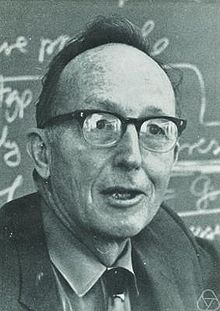
\includegraphics[scale=0.6]{maclane}

Saunders Mac Lane
\end{center}

\begin{center}
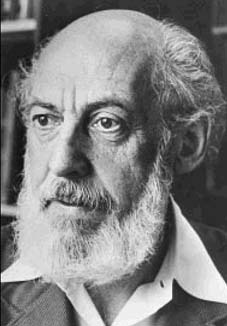
\includegraphics[scale=0.6]{eilenberg}

Samuel Eilenberg
\end{center}

\begin{center}
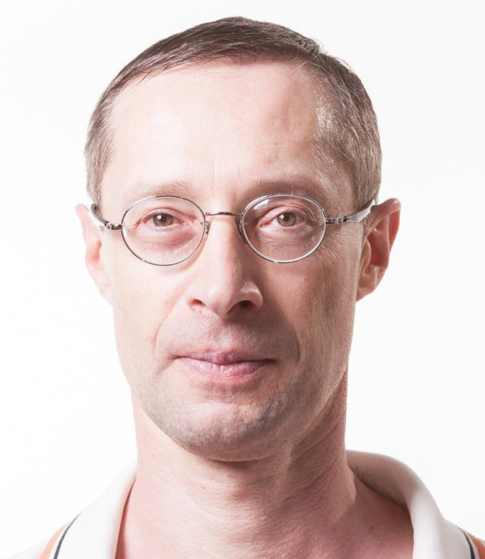
\includegraphics[scale=0.3]{moggi}
\end{center}

Eugenio Moggi is a professor of computer science at the University of Genoa, Italy.
He first described the general use of monads to structure programs.

\begin{center}

\includegraphics[scale=0.45]{wadler}
\end{center}

Philip Lee Wadler is an American computer scientist known for his contributions to programming language design and type theory.

\subsection{Definizione}

Quella seguente è una possibile definizione che si può trovare in rete:

Una monade $M$ nella categoria $\mathcal{C}$ è un endofuntore di $\mathcal{C}$ con due operazioni aggiuntive

\begin{code}
interface Monad<F> extends Functor<F> {
  of: <A>(a: A) => M<A>
  chain: <A, B>(f: (a: A) => M<B>, ma: M<A>) => M<B>
}
\end{code}

Inoltre devono valere le seguenti leggi

\begin{center}
\bgroup
\def\arraystretch{1.5}
\begin{tabular}{ |c|p{10cm}| }
\hline
Left identity & \texttt{chain(f, of(x)) = f(x)} \\
\hline
Right identity & \texttt{chain(of, x) = x} \\
\hline
Associativity & \texttt{chain(g, chain(f, ma)) = chain(x => chain(g, f(x)), mx)} \\
\hline
\end{tabular}
\egroup
\end{center}

Possibili sinonimi di \texttt{of}\footnote{Nome contenuto nella specifica https://github.com/fantasyland/fantasy-land} sono \texttt{return}, \texttt{pure} e \texttt{point}, sinonimi di \texttt{chain} sono \texttt{bind} e \texttt{flatMap}.

\begin{itemize}
  \item perché ci sono esattamente quelle due funzioni?
  \item perché hanno quelle firme?
  \item perché devono valere quelle leggi?
\end{itemize}

Per rispondere a queste domande introduciamo un concetto equivalente a quello di monade: le \emph{categorie di Kleisli}

\subsection{Categorie di Kleisli}

\begin{center}
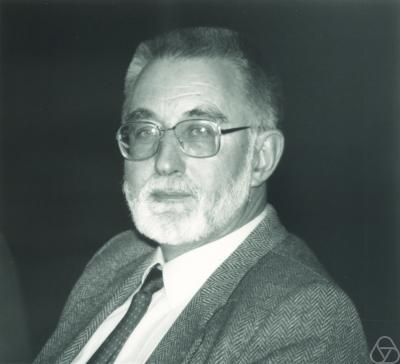
\includegraphics[scale=0.5]{kleisli}

Heinrich Kleisli (Swiss mathematician)
\end{center}

Sia $M$ un endofuntore nella categoria $\mathcal{C}$ e si considerino i due morfismi $g: A \rightarrow M(B)$, $f: B \rightarrow M(C)$

\[
\xymatrixrowsep{3cm}
\xymatrixcolsep{3cm}
\xymatrix{
  & M(B) & M(C) \\
  A \ar[ur]^g & B \ar[ur]^f & C
}
\]

Chiamiamo \emph{Kleisli arrow} i morfismi come $g$ ed $f$, ovvero i morifismi il cui target è l'immagine di $M$.

\begin{demo}
Una Kleisli arrow $f: A \rightarrow M(B)$ può essere interpretata come un programma che accetta un input di tipo $A$ e che produce un output di tipo $B$ insieme ad un effetto di tipo $M$
\end{demo}

Le Kleisli arrows $g: A \rightarrow M(B)$, $f: B \rightarrow M(C)$ non compongono rispetto a $\circ$, l'operazione di composizione della categoria $\mathcal{C}$,
poichè $M(B)$ è diverso da $B$.

Si consideri allora la seguente costruzione $K_{\mathcal{C}}$

\[
\xymatrixrowsep{3cm}
\xymatrixcolsep{3cm}
\xymatrix{
  A \ar[r]^{g'} & B \ar[r]^{f'} & C
}
\]

ove

\begin{itemize}
  \item $A, B, C, \ldots$ sono gli oggetti di $\mathcal{C}$
  \item esiste una morfismo $m': A \rightarrow B$ in $K_{\mathcal{C}}$ se e solo se esiste un morfismo $m: A \rightarrow M(B)$ in $\mathcal{C}$
\end{itemize}

\begin{demo}
Definire una buona operazione di composizione per le Kleisli arrow in $\mathcal{C}$, indichiamola con $\bullet$, vuol dire imporre che $K_{\mathcal{C}}$ sia una categoria.
\end{demo}

Per dimostrare che $K_{\mathcal{C}}$ è una categoria dobbiamo definire una operazione di composizione, indichiamola con $\diamond$,
e dimostrare che valgono le leggi categoriali (identità sinistra, identità destra e associatività).

\paragraph{Composizione}

Se $K_{\mathcal{C}}$ è una categoria allora deve esistere un morfismo $f' \diamond g': A \rightarrow C$.
Ma allora il corrispondente morfismo $f \bullet g$ in $\mathcal{C}$ deve avere come sorgente $A$ e come target $M(C)$, ovvero $h: A \rightarrow M(C)$.
Proviamo a costruirlo

\[
\xymatrixrowsep{3cm}
\xymatrixcolsep{3cm}
\xymatrix{
  && M(M(C)) \ar[d]^{flatten} \\
  & M(B) \ar[ur]^{M(f)} & M(C) \\
  A \ar[ur]^g \ar@{-->}[urr]^{f \bullet g} & B \ar[ur]^f & C \\
  A \ar[r]^{g'} \ar@/_1cm/[rr]_{f' \diamond g'} & B \ar[r]^{f'} & C
}
\]

$$
f \bullet g = flatten \circ M(f) \circ g
$$

\paragraph{Morfismi identità}

Se $K_{\mathcal{C}}$ è una categoria allora per ogni $A$ deve esistere un morfismo $1'_A: A \rightarrow A$,
perciò deve esistere un morfismo $\eta_A: A \rightarrow M(A)$ in $\mathcal{C}$.

\[
\xymatrixrowsep{3cm}
\xymatrixcolsep{3cm}
\xymatrix{
  M(A) \\
  A \ar[u]_{\eta_A} \\
  A \ar@(ul,ur)^{1'_A}
}
\]

\paragraph{Identità sinistra e destra}

\[
\xymatrixrowsep{3cm}
\xymatrixcolsep{3cm}
\xymatrix{
  & M(M(C)) \ar@/_-0.5cm/[d]^{flatten} \\
  M(B) \ar[ur]^{M(f)} & M(C) \ar@/_-0.5cm/[u]^{M(\eta_C)} \\
  B \ar[u]^{\eta_B} \ar[ur]^f & C \ar[u]^{\eta_C} \\
  B \ar@(ul,ur)^{1'_B} \ar[r]^{f'} & C \ar@(ul,ur)^{1'_C}
}
\]

\begin{itemize}
  \item $1'_B \diamond f' = f'$ implica $\eta_B \bullet f = f$ ovvero \texttt{chain(f, of(b)) = f(b)}
  \item $f' \diamond 1'_C = f'$ implica $f \bullet \eta_C = f$ ovvero \texttt{chain(of, c) = c}
\end{itemize}

\paragraph{Associatività}

\[
\xymatrixrowsep{3cm}
\xymatrixcolsep{3cm}
\xymatrix{
  & M(B) & M(C) & M(D) \\
  A \ar[ur]^g \ar@{-->}[urr]^{f \bullet g} & B \ar[ur]^f \ar@{-->}[urr]^{h \bullet f} & C \ar[ur]^h & D \\
  A \ar[r]^{g'} \ar@/_1cm/[rr]_{f' \diamond g'} & B \ar[r]^{f'} \ar@/_1cm/[rr]_{f' \diamond g'} & C \ar[r]^{h'} & D
}
\]

$$
h \diamond (f \diamond g) = (h \diamond f) \diamond g
$$

ovvero

\begin{center}
\texttt{chain(h, chain(f, mb)) = chain(b => chain(h, f(b)), mb)}
\end{center}

\subsection{Ricapitolando}

\paragraph{Perché le categorie sono importanti?}

Perché sono alla base del concetto di composizione e di monade e modellano i linguaggi di programmazione.

\paragraph{Cos'è una monade?}

$M$ è una monade quando i programmi con effetti $A \rightarrow M(B)$ costituiscono i morfismi di una categoria.

\paragraph{Perché le monadi sono importanti?}

Perché se $M$ è una monade posso comporre i programmi con effetti $A \rightarrow M(B)$ tra loro.

\paragraph{Una monade per ogni occasione.}

\begin{itemize}
  \item eseguire un'azione sincrona? monade \texttt{IO}
  \item eseguire computazioni asincrone? monade \texttt{Task}
  \item leggere una configurazione? monade \texttt{Reader}
  \item scrivere su un log? monade \texttt{Writer}
  \item gestire lo stato? monade \texttt{State}
  \item gestire gli errori? monade \texttt{Option} o \texttt{Either}
  \item gestire risultati non deterministici? monade \texttt{Array}
\end{itemize}

\subsection{Esempi}

\begin{example}
Istanza per \texttt{Identity<A>}

\begin{code}
const of = <A>(a: A) => new Identity(a)

class Identity<A> {
  ...
  chain<B>(f: (a: A) => Identity<B>): Identity<B> {
    return f(this.value)
  }
}
\end{code}
\end{example}

\begin{example}
Istanza per \texttt{Option<A>}

\begin{code}
const of = some

class None<A> {
  ...
  chain<B>(f: (a: A) => Option<B>): Option<B> {
    return none
  }
}

class Some<A> {
  ...
  chain<B>(f: (a: A) => Option<B>): Option<B> {
    return f(this.value)
  }
}
\end{code}
\end{example}

\begin{example}
Istanza per \texttt{Either<L, A>}

\begin{code}
const of = right

class Left<L, A> {
  ...
  chain<B>(f: (a: A) => Either<L, B>): Either<L, B> {
    return left(this.value)
  }
}

class Right<L, A> {
  ...
  chain<B>(f: (a: A) => Either<L, B>): Either<L, B> {
    return f(this.value)
  }
}
\end{code}
\end{example}

\begin{example}
Istanza per \texttt{Array<A>}

\begin{code}
const monadArray = {
  ...
  chain: <A, B>(
    f: (a: A) => Array<B>,
    fa: Array<A>
  ): Array<B> =>
    fa.reduce((acc, a) => acc.concat(f(a)), [] as Array<B>)
}
\end{code}
\end{example}

\begin{example}
Istanza per \texttt{IO<A>}

\begin{code}
const of = <A>(a: A): IO<A> => new IO(() => a)

class IO<A> {
  ...
  chain<B>(f: (a: A) => IO<B>): IO<B> {
    return new IO(() => f(this.run()).run())
  }
}
\end{code}
\end{example}

\begin{example}
Istanza per \texttt{Task<A>}

\begin{code}
const of = <A>(a: A): Task<A> =>
  new Task(() => Promise.resolve(a))

class Task<A> {
  ...
  chain<B>(f: (a: A) => Task<B>): Task<B> {
    return new Task(() => this.run().then(a => f(a).run()))
  }
}
\end{code}
\end{example}

\begin{exercise}
Sia

\begin{code}
type Tuple<L, A> = [L, A]
\end{code}

definire una istanza di monade.
\end{exercise}

\subsection{\texttt{Task} vs \texttt{Promise}}

\texttt{Task} è una astrazione simile a \texttt{Promise}, la differenza chiave è che \texttt{Task} rappresenta una computazione asincrona
mentre \texttt{Promise} rappresenta solo un risultato (ottenuto in maniera asincrona).

Se abbiamo un \texttt{Task}

\begin{itemize}
  \item possiamo far partire la computazione che rappresenta (per esempio una richiesta network)
  \item possiamo scegliere di non far partire la computazione
  \item possiamo farlo partire più di una volta (e potenzialmente ottenere risultati diversi)
  \item mentre la computazione si sta svolgendo, possiamo notificagli che non siamo più interessati al risultato e la computazione può scegliere di terminarsi da sola
  \item quando la computazione finisce otteniamo il risultato
\end{itemize}

Se abbiamo una \texttt{Promise}

\begin{itemize}
  \item la computazione si sta già svolgendo (o è addirittura già finita) e non abbiamo controllo su questo
  \item quando è disponible otteniamo il risultato
  \item due consumatori della stessa \texttt{Promise} ottengono lo stesso risultato
\end{itemize}

\subsection{Derivazione di \texttt{map}}

L'operazione \texttt{map} può essere derivata da \texttt{chain} e \texttt{of}

\begin{code}
const map = <A, B>(f: (a: A) => B) => (
  fa: Option<A>
): Option<B> => fa.chain(a => of(f(a)))
\end{code}

\subsection{Derivazione di \texttt{ap}}

L'operazione \texttt{ap} può essere derivata da \texttt{chain} e \texttt{map}

\begin{code}
const ap = <A, B>(fab: Option<(a: A) => B>) => (
  fa: Option<A>
): Option<B> => fab.chain(f => fa.map(f))
\end{code}

\subsection{Esecuzione parallela e sequenziale}

\begin{code}
// par-seq.ts

const liftA2 = <A, B, C>(
  f: (a: A) => (b: B) => C
): ((
  fa: Task<A>
) => (fb: Task<B>) => Task<C>) => fa => fb =>
  fb.ap(fa.map(f))

const sumTasks = liftA2(
  (a: number) => (b: number): number => a + b
)

const delay = (n: number) => <A>(a: A): Task<A> =>
  new Task(
    () =>
      new Promise(resolve => {
        setTimeout(() => resolve(a), n)
      })
  )

const oneSec = delay(1000)

sumTasks(oneSec(1))(oneSec(3))
  .run()
  .then(x => console.log(x))
\end{code}

Eseguendo il codice mostrando il tempo di esecuzione otteniamo
\footnote{\texttt{ts-node} è un wrapper di \texttt{node} in grado di eseguire codice TypeScript}

\begin{code}
$ time ts-node par-seq.ts

3

real    0m1.383s
user    0m0.327s
sys     0m0.058s
\end{code}

Il che mostra che le computazioni asincrone vengono eseguite in modo concorrente.

Se però come implementazione di \texttt{ap} per \texttt{Task} scegliamo quella derivata da \texttt{chain} otteniamo

\begin{code}
$ time ts-node par-seq.ts

3

real    0m2.402s
user    0m0.342s
sys     0m0.063s
\end{code}

Che cosa è successo? La spiegazione è che l'implementazione di \texttt{ap} derivata da \texttt{chain} è sempre \textbf{sequenziale}.

\subsection{Trasparenza referenziale}

Vediamo ora come, grazie alla trasparenza referenziale e al concetto di monade, possiamo manipolare i programmi programmaticamente.

Ecco un piccolo programma che legge / scrive su un file

\begin{code}
//
// funzioni di libreria
//

const readFile = (filename: string): IO<string> =>
  new IO(() => fs.readFileSync(filename, 'utf-8'))

const writeFile = (
  filename: string,
  data: string
): IO<void> =>
  new IO(() =>
    fs.writeFileSync(filename, data, { encoding: 'utf-8' })
  )

const log = (message: string): IO<void> =>
  new IO(() => console.log(message))

//
// programma
//

const program1 = readFile('file.txt')
  .chain(log)
  .chain(() => writeFile('file.txt', 'hello'))
  .chain(() => readFile('file.txt'))
  .chain(log)
\end{code}

L'azione

\begin{code}
readFile('file.txt').chain(log)
\end{code}

è ripetuta due volte nel programma, ma dato che vale la trasparenza referenziale
possiamo mettere a fattor comune l'azione assegnandone l'espressione ad una costante

\begin{code}
const read = readFile('file.txt').chain(log)

const program2 = read
  .chain(() => writeFile('file.txt', 'foo'))
  .chain(() => read)
\end{code}

Possiamo anche definire un combinatore e sfruttarlo per rendere più compatto il codice

\begin{code}
// a -> b -> a
const interleave = <A, B>(a: IO<A>, b: IO<B>): IO<A> =>
  a.chain(() => b).chain(() => a)

const program3 = interleave(
  read,
  writeFile('file.txt', 'foo')
)
\end{code}

\begin{demo}
\begin{center}
\textbf{DEMO}

\texttt{game.ts}
\end{center}
\end{demo}

\subsection{Le monadi non compongono}

In generale le monadi non compongono, ovvero date due istanze di monade, una per \texttt{M<A>} e una per \texttt{N<A>},
allora a \texttt{M<N<A>>} non è detto che possa ancora essere associata una istanza di monade.

Che non compongano in generale però non vuol dire che non esistano dei casi particolari ove questo succede.

Vediamo qualche esempio, se \texttt{M} ha una istanza di monade allora ammettono una istanza di monade i seguenti tipi

\begin{itemize}
  \item \texttt{OptionT<M, A> = M<Option<A>>}
  \item \texttt{EitherT<M, L, A> = M<Either<L, A>>}
\end{itemize}

Notate come questi tipi collassino in quelli già conosciuti quando il type constructor \texttt{M} è \texttt{Identity}

\begin{itemize}
  \item \texttt{Option<A> = OptionT<Identity, A>}
  \item \texttt{Either<L, A> = EitherT<Identity, L, A>}
\end{itemize}

\texttt{OptionT} e \texttt{EitherT} sono esempi di \emph{monad transformer}.

\newpage

\section{Algebraic Data Types}

Un \emph{Algebraic Data Type} (o ADT) è un tipo composto da product e/o sum types, anche innestati.

\subsection{Product types}

\begin{definition}
Un product type è una collezione di tipi $A_i$ indicizzati da un insieme $I$.
\end{definition}

Un product type è isomorfo\footnote{Due insiemi $A$ e $B$ sono isomorfi se esiste una funzione $f: A \rightarrow B$ iniettiva e suriettiva,
ovvero se esiste una funzione $f^{-1}: B \rightarrow A$, detta \emph{funzione inversa} di $f$, tale che $f \circ f^{-1} = identity$}
al prodotto cartesiano $\prod_i A_i$.

Esponenti notevoli di questa famiglia sono le $n$-tuple, ove $I$ è un intervallo non vuoto dei numeri naturali
\footnote{$\{0\}$ per \texttt{Tuple1}, $\{0, 1\}$ per \texttt{Tuple2}, $\{0, 1, 2\}$ per \texttt{Tuple2}}

\begin{code}
type Tuple1 = [string]
type Tuple2 = [string, number]
type Tuple3 = [string, number, boolean]
\end{code}

e i record, ove $I$ è una collezione di label
\footnote{$\{ "name", "age" \}$ per \texttt{Person}}

\begin{code}
type Person = {
  name: string,
  age: number
}
\end{code}

\texttt{Tuple2} e \texttt{Person} sono isomorfi tra loro e al prodotto cartesiano $string \times number$.

$$
f: \texttt{Tuple2} \rightarrow \texttt{Person}
$$

$$
f(\texttt{[name, age]}) = \texttt{\{ name, age  \}}
$$

$$
f^{-1}: \texttt{Person} \rightarrow \texttt{Tuple2}
$$

$$
f^{-1}(\texttt{\{ name, age  \}}) = \texttt{[name, age]}
$$

L'isomorfismo è evidente se si implementa \texttt{Person} con una classe

\begin{code}
class Person {
  name: string,
  age: number
  constructor(name: string, age: number) {
    this.name = name
    this.age = age
  }
}
\end{code}

in cui \texttt{constructor} realizza la funzione $f$.

Perché si chiamano product types? Se indichiamo con $\|A\|$, detta \emph{cardinalità} o \emph{ordine} di $A$, il numero di elementi
dell'insieme $A$ è facile convincersi che vale la seguente formula

$$
\|A \times B\| = \|A\| * \|B\|
$$

ovvero la cardinalità del prodotto cartesiano è il prodotto delle cadinalità.

\begin{code}
type Hour = 1 | 2 | 3 | 4 | 5 | 6 | 7 | 8 | 9 | 10 | 11 | 12
type Period = 'AM' | 'PM'
type Clock = [Hour, Period]
\end{code}

Il tipo \texttt{Clock} ha $12 * 2 = 24$ abitanti.

\subsection{Sum types}

Così come i product types sono analoghi ai prodotti cartesiani di insiemi, i sum types sono analoghi alle unioni di insiemi disgiunti

\begin{code}
type Action =
  | { type: 'INCREMENT' }
  | { type: 'DECREMENT' }
\end{code}

Product types e sum types possono essere mischiati

\begin{code}
type Action =
  | { type: 'ADD_TODO'; text: string }
  | {
      type: 'UPDATE_TODO'
      id: number
      text: string
      completed: boolean
    }
  | { type: 'DELETE_TODO'; id: number }
\end{code}

Il tipo \texttt{Array<A>} può essere interpretato come sum type

\begin{code}
type Array<A> = [] | [A] | [A, A] | [A, A, A] | ...
\end{code}

\begin{example}
Linked lists\footnote{È possibile definire una istanza di funtore per \texttt{List<A>}

\begin{code}
const map = <A, B>(f: (a: A) => B) => (
  fa: List<A>
): List<B> => {
  switch (fa.type) {
    case 'Nil':
      return { type: 'Nil' }
    case 'Cons':
      return {
        type: 'Cons',
        head: f(fa.head),
        tail: map(f)(fa.tail)
      }
  }
}
\end{code}
}

\begin{code}
type List<A> =
  | { type: 'Nil' }
  | { type: 'Cons', head: A, tail: List<A> }
\end{code}
\end{example}

\begin{example}
Binary trees\footnote{È possibile definire una istanza di funtore per \texttt{Tree<A>}

\begin{code}
const map = <A, B>(f: (a: A) => B) => (
  fa: Tree<A>
): Tree<B> => {
  switch (fa.type) {
    case 'Empty':
      return { type: 'Empty' }
    case 'Node':
      return {
        type: 'Node',
        left: map(f)(fa.left),
        value: f(fa.value),
        right: map(f)(fa.right)
      }
  }
}
\end{code}
}

\begin{code}
type Tree<A> =
  | { type: 'Empty' }
  | {
      type: 'Node'
      left: Tree<A>
      value: A
      right: Tree<A>
    }
\end{code}
\end{example}

Perché si chiamano sum types? È facile convincersi che la cadinalità di un sum type è la somma delle cardinalità dei suoi membri

$$
\|A | B\| = \|A\| + \|B\|
$$

Il tipo \texttt{Option<boolean>} ha $1 + 2 = 3$ abitanti.

\newpage

\section{Make impossible states irrepresentable}

Vediamo un'altra tecnica per ottenere type safety, questa volta addirittura per costruzione.

Sappiamo che la funzione \texttt{head} è parziale

\begin{code}
const head = <A>(xs: Array<A>): A => xs[0]
\end{code}

e che per renderla totale occorre modificare il codominio

\begin{code}
const head = <A>(xs: Array<A>): Option<A> =>
  xs.length > 0 ? some(xs[0]) : none
\end{code}

Tuttavia questo ci obbliga ad usare \texttt{Option}.

Un'altra opzione è quella di cambiare il dominio invece che estendere il codominio

\subsection{Il tipo \texttt{NonEmptyArray}}

\begin{code}
class NonEmptyArray<A> {
  constructor(readonly head: A, readonly tail: Array<A>) {}
}

const head = <A>(fa: NonEmptyArray<A>): A => fa.head
\end{code}

\subsection{Il tipo \texttt{Zipper}}

Supponiamo di dover modellare la seguente struttura dati

\begin{quote}
una lista non vuota di elementi di cui uno è considerato la selezione corrente
\end{quote}

Un modello semplice potrebbe essere questo

\begin{code}
type Selection<A> = {
  items: Array<A>
  current: number
}
\end{code}

Tuttavia questo modello ha diversi difetti

\begin{itemize}
  \item la lista può essere vuota
  \item l'indice può essere out of range
\end{itemize}

Uno \texttt{Zipper} invece è un modello perfetto e type safe per il problema

\begin{code}
type Zipper<A> = {
  prev: Array<A>
  current: A
  next: Array<A>
}
\end{code}

\subsection{Smart constructors}

Consideriamo la funzione \texttt{inverse}

\begin{code}
const inverse = (x: number): Option<number> =>
  x === 0 ? none : some(1 / x)
\end{code}

Un altro modo per ottenere lo stesso grado di type safety senza avere una funzione parziale è l'utilizzo degli \emph{smart constructors}.

In pratica si fa in modo che \texttt{Option} non compaia a valle, nel codominio di \texttt{inverse},
ma a monte, in fase di creazione dell'input \texttt{x}.

In generale, se voglio rappresentare un raffinamento di un tipo \texttt{A} (come per esempio il fatto che sia un numero diverso da zero),
faccio in modo che il suo costruttore non sia invocabile al di fuori del suo modulo e fornisco un costruttore alternativo
che però restituisce una \texttt{Option<A>} dato che a runtime verrà effettuato il controllo che il raffinamento sussista davvero.

\begin{code}
class NonZero {
  // private
  private constructor(readonly value: number) {}
  // smart constructor
  static create(value: number): Option<NonZero> {
    return value === 0 ? none : some(new NonZero(value))
  }
}

const inverse = (x: NonZero): number => 1 / x.value
\end{code}

In questo modo spesso si spingono i controlli a runtime là dove dovrebbe essere il loro posto naturale: ai confini del sistema,
dove vengono fatte tutte le validazioni dell'input.

\newpage

\section{Foldable}

È possibile generalizzare la funzione \texttt{reduce} definita per \texttt{Array}?

\begin{code}
reduce: <A, B>(fa: Array<A>, b: B, f: (b: B, a: A) => B) => B
\end{code}

La risposta è affermativa e conduce al concetto di \texttt{Foldable}.

\texttt{Foldable} rappresenta una struttura che può essere ridotta tramite una operazione \texttt{reduce}
(sinonimi: \texttt{reduceLeft}, \texttt{foldLeft}, \texttt{foldl})

\subsection{Definizione}

\begin{code}
interface Foldable<F> {
  reduce: <A, B>(fa: F<A>, b: B, f: (b: B, a: A) => B) => B
}
\end{code}

Definizioni equivalenti\footnote{ovvero ogni operazione può essere derivata da una qualsiasi delle altre} di \texttt{Foldable}
coinvolgono l'operazione

\begin{code}
reduceRight: <A, B>(fa: F<A>, b: B, f: (a: A, b: B) => B) => B
\end{code}

(sinonimi: \texttt{foldRight}, \texttt{foldr}) oppure l'operazione

\begin{code}
foldMap: <M>(M: Monoid<M>) =>
  <A>(fa: F<A>, f: (a: A) => M) => M
\end{code}

\begin{exercise}
Mostrare che le definizioni tramite \texttt{reduce}, \texttt{foldr} e \texttt{foldMap} sono equivalenti.
\end{exercise}

Un modo per afferrare il concetto di \texttt{Foldable} è che una struttura che ammette una sua istanza
è in grado di essere rappresentata sotto forma di array.

Infatti è possibile definire la seguente funzione

\begin{code}
const toArray = <F>(F: Foldable<F>) => <A>(fa: F<A>): Array<A>
\end{code}

\begin{exercise}
Perché? Suggerimento: usare \texttt{foldMap}.
\end{exercise}

È importante notare che affinchè sia possibile scrivere una istanza di \texttt{Foldable} è necessario che la produzione di valori
di tipo \texttt{A} abbia un ordine deterministico dato che la riduzione passa attraverso la funzione

\begin{code}
f: (b: B, a: A) => B
\end{code}

\begin{exercise}
\texttt{Option<A>} ammette una istanza di \texttt{Foldable}, qual'è la sua rappresentazione come array?
\end{exercise}

\subsection{Differenze tra \texttt{reduceLeft} e \texttt{reduceRight}}

\texttt{reduceLeft} è \emph{associativa a sinistra}

$$
reduce(b, f, [x_1, x_2, \ldots , x_n])  == f( \ldots f(f(b, x_1), x_2), \ldots x_n)
$$

mentre \texttt{reduceRight} è \emph{associativa a destra}

$$
reduceRight(b, f, [x_1, x_2, \ldots , x_n])  == f(f( \ldots f(b, x_n) \ldots , x_2), x_1)
$$

\begin{example}
Ridurre \texttt{Array<string>} tramite concatenazione

\begin{code}
reduce(["a", "b", "c"], "", (b, a) => b + a) // "abc"

reduceRight(["a", "b", "c"], "", (a, b) => b + a) // "cba"
\end{code}
\end{example}

\subsection{\texttt{Foldable} e \texttt{Functor}}

\texttt{Foldable} e \texttt{Functor} sono indipendenti, ovvero esistono strutture che ammettono una istanza di \texttt{Foldable} ma non una di
\texttt{Functor} e viceversa.

\texttt{Task<A>} ammette una istanza di \texttt{Functor} ma non di \texttt{Foldable}.

La seguente struttura dati

\begin{code}
class Weird<A> {
  constructor(
    readonly value: A,
    readonly endo: (a: A) => A
  ) {}
}
\end{code}

ammette una istanza di \texttt{Foldable}

\begin{code}
const reduce = <A, B>(
  fa: Weird<A>,
  b: B,
  f: (b: B, a: A) => B
): B => f(b, fa.endo(fa.value))
\end{code}

ma non di \texttt{Functor} perché \texttt{A} compare in posizione controvariante.

\subsection{Esempi}

\begin{example}
Istanza per \texttt{Identity<A>}

\begin{code}
const reduce = <A, B>(
  fa: Identity<A>,
  b: B,
  f: (b: B, a: A) => B
): B => f(b, fa.value)
\end{code}
\end{example}

\begin{example}
Istanza per \texttt{Option<A>}

\begin{code}
const reduce = <A, B>(
  fa: Option<A>,
  b: B,
  f: (b: B, a: A) => B
): B => (isSome(fa) ? f(b, fa.value) : b)
\end{code}
\end{example}

\begin{example}
Istanza per \texttt{Either<L, A>}

\begin{code}
const reduce = <L, A, B>(
  fa: Either<L, A>,
  b: B,
  f: (b: B, a: A) => B
): B => (isRight(fa) ? f(b, fa.value) : b)
\end{code}
\end{example}

\begin{example}
Istanza per \texttt{Array<A>}

\begin{code}
const reduce = <A, B>(
  fa: Array<A>,
  b: B,
  f: (b: B, a: A) => B
): B => fa.reduce(f, b)
\end{code}
\end{example}

\begin{exercise}
Definire una istanza di \texttt{Foldable} per \texttt{Tree<A>}

\begin{code}
type Tree<A> =
  | { type: 'Empty' }
  | {
      type: 'Node'
      left: Tree<A>
      value: A
      right: Tree<A>
    }
\end{code}
\end{exercise}

\begin{exercise}
È possibile definire una istanza di \texttt{Foldable} per \texttt{Set<A>}?
\end{exercise}

\begin{exercise}
È possibile definire una istanza di \texttt{Foldable} per \texttt{IO<A>}?
\end{exercise}

\subsection{Funzioni associate a \texttt{Foldable}}

\begin{function}
Una generalizzazione della funzione \texttt{fold} che lavora con gli array

\begin{code}
fold: <F, M>(F: Foldable<F>, M: Monoid<M>) => (fa: F<M>) => M
\end{code}
\end{function}

\begin{function}
Simile a \texttt{reduce} ma il risultato è incapsulato in una monade

\begin{code}
foldM: <F, M>(F: Foldable<F>, M: Monad<M>) => <A, B>(
  f: (b: B, a: A) => M<B>,
  b: B,
  fa: F<A>
) => M<B>
\end{code}
\end{function}

\begin{function}
Attraversa una struttura dati eseguendo un qualche effetto codificato da una funtore applicativo per ogni valore, ignorando il risultato finale

\begin{code}
traverse_: <M, F>(
  M: Applicative<M>,
  F: Foldable<F>
) => <A, B>(
  f: (a: A) => M<B>,
  fa: F<A>
) => M<void>
\end{code}
\end{function}

\begin{function}
Esegue tutti gli effetti contenuti in una struttura dati nell'ordine dato dall'istanza di \texttt{Foldable}, ignorando il risultato finale

\begin{code}
sequence_: <M, F>(
  M: Applicative<M>,
  F: Foldable<F>
) => <A>(fa: F<M<A>>): M<void>
\end{code}
\end{function}

\begin{observation}
\texttt{sequence\_} può essere derivato da \texttt{traverse\_}

\begin{code}
sequence_(M, F)(x) = traverse_(M, F)(identity, x)
\end{code}
\end{observation}

\subsection{I \texttt{Foldable} compongono}

Dati due type constructor \texttt{F<A>} e \texttt{G<A>} tali che ammettono una istanza di \texttt{Foldable}, allora la composizione \texttt{F<G<A>>}
ammette una istanza di \texttt{Foldable}.

\begin{example}
\texttt{ArrayOption<A>}

\begin{code}
import { option } from "fp-ts/lib/Option"

const reduce = <A, B>(
  fa: ArrayOption<A>,
  b: B,
  f: (b: B, a: A) => B
): B => fa.value.reduce((b, o) => option.reduce(o, b, f), b)

reduce(
  new ArrayOption([some("a"), none, some("b")]),
  "",
  (b, a) => b + a
) // "ab"
\end{code}
\end{example}

\begin{demo}
\begin{center}
\textbf{DEMO}

\texttt{BinaryTree.ts} \\
\texttt{wizard.ts}
\end{center}
\end{demo}

\newpage

\section{Traversable}

Data una istanza di \texttt{Applicative} per \texttt{F} é possibile definire la seguente funzione

\begin{code}
traverseA: <F>(F: Applicative<F>) => <A, B>(
  ta: Array<A>,
  f: (a: A) => F<B>
) => F<Array<B>>
\end{code}

\begin{exercise}
(Difficile) Implementare la funzione \texttt{traverseA}
\end{exercise}

È possibile generalizzare la funzione \texttt{traverseA} sopra definita per strutture dati diverse da \texttt{Array}?

La risposta è affermativa e conduce al concetto di \texttt{Traversable}

\subsection{Definizione}

\texttt{Traversable} rappresenta una struttura che può essere attraversata eseguendo una azione per ogni elemento.

\begin{code}
interface Traversable<T> extends Functor<T>, Foldable<T> {
  traverse: <F>(F: Applicative<F>) =>
    <A, B>(ta: T<A>, f: (a: A) => F<B>) => F<T<B>>
}
\end{code}

\begin{observation}
È importante notare che, al contrario di quanto succede con \texttt{Foldable} in cui la struttura originale viene persa,
con \texttt{Traversable} la struttura viene preservata.
\end{observation}

Alternativamente \texttt{Traversable} può essere definita tramite la funzione

\begin{code}
sequence: <F>(F: Applicative<F>) => <A>(tfa: T<F<A>>) => F<T<A>>
\end{code}

Una istanza di \texttt{Traversable} deve soddisfare le seguenti leggi

\begin{center}
\bgroup
\def\arraystretch{1.5}
\begin{tabular}{ |c|p{10cm}| }
\hline
naturality & \texttt{at(traverse(F1)(f, ta)) = traverse(F2)(compose(at, f), ta)} per ogni \emph{applicative transformation} \texttt{at} \\
\hline
identity & \texttt{traverse(F)(a => new Identity(a), ta) = new Identity(ta)} \\
\hline
composition & \texttt{traverse(F)(a => compose(fa => A.map(g, fa), f), ta) = F.map(tfa => traverse(A)(g, tfa), traverse(F)(f, ta))} \\
\hline
\end{tabular}
\egroup
\end{center}

Una \emph{applicative transformation} è una funzione con la seguente firma

\begin{code}
at: (F: Applicative<F>, g: Applicative<G>) =>
  <A>(fa: F<A>) => G<A>
\end{code}

\subsection{Esempi}

\begin{example}
Istanza per \texttt{Identity<A>}

\begin{code}
function traverse<F>(
  F: Applicative<F>
): <A, B>(
  ta: Identity<A>,
  f: (a: A) => F<FB>
) => F<Identity<B>> {
  return (ta, f) => F.map(identity.of, f(ta.value))
}
\end{code}
\end{example}

\begin{example}
Istanza per \texttt{Array<A>}

\begin{code}
const snoc = <A>(as: Array<A>) => (a: A): Array<A> =>
  as.concat([a])

function traverse<F>(
  F: Applicative<F>
): <A, B>(
  ta: Array<A>,
  f: (a: A) => F<B>
) => F<Array<B>> {
  const snocLifted = liftA2(F)(snoc)
  return (ta, f) =>
    reduce(ta, F.of([]), (fab, a) => snocLifted(fab)(f(a)))
}
\end{code}
\end{example}

\begin{exercise}
Definire una istanza di \texttt{Traversable} per \texttt{Option<A>}
\end{exercise}

\begin{exercise}
Definire una istanza di \texttt{Traversable} per \texttt{Either<L, A>}
\end{exercise}

\begin{exercise}
È possibile definire una istanza di \texttt{Traversable} per \texttt{Task<A>}?
\end{exercise}

\subsection{La funzione \texttt{sequence}}

Da \texttt{traverse} è possibile derivare la seguente funzione \footnote{e viceversa}

\begin{code}
sequence: <F, T>(F: Applicative<F>, T: Traversable<T>) =>
  (tfa: T<F<A>>) => F<T<A>>
\end{code}

Ecco alcuni esempi di come lavora la funzione \texttt{sequence}

\begin{center}
\bgroup
\def\arraystretch{1.5}
\begin{tabular}{ |c|c| }
\hline
From & To \\
\hline
\texttt{Array<Option<A>>} & \texttt{Option<Array<A>>} \\
\hline
\texttt{Either<L, IO<A>>} & \texttt{IO<Either<L, A>>} \\
\hline
\texttt{Array<Either<L, A>>} & \texttt{Either<L, Array<A>>} \\
\hline
\texttt{Either<L, Task<A>>} & \texttt{Task<Either<L, A>>} \\
\hline
\end{tabular}
\egroup
\end{center}

\subsection{I \texttt{Traversable} compongono}

Ovvero se sia \texttt{F<A>} che \texttt{G<A>} ammettono una istanza di \texttt{Traversable}, allora \texttt{F<G<A>>} ammette una istanza di \texttt{Traversable}

\begin{example}
\texttt{ArrayOption<A>}

\begin{code}
import { Applicative1 } from "fp-ts/lib/Applicative"
import { URIS, Type } from "fp-ts/lib/HKT"
import { task } from "fp-ts/lib/Task"
import { traverse as t } from "fp-ts/lib/Traversable"

const traverse = <F extends URIS>(F: Applicative1<F>) => <
  A,
  B
>(
  ta: ArrayOption<A>,
  f: (a: A) => Type<F, B>
): Type<F, ArrayOption<B>> => {
  return F.map(
    t(F, array)(ta.value, o => t(F, option)(o, f)),
    a => new ArrayOption(a)
  )
}

traverse(task)(
  new ArrayOption([some('foo'), none, some('quux')]),
  a => task.of(a.length)
)
  .run()
  .then(x => console.log(x))
/*
ArrayOption([some(3), none, some(4)])
*/
\end{code}
\end{example}

\begin{demo}
\begin{center}
\textbf{DEMO}

\texttt{BinaryTree.ts} \\
\texttt{traversable.ts}
\end{center}
\end{demo}

\newpage

\section{Alternative}

\subsection{\texttt{Alt}}

\begin{code}
interface Alt<F> extends Functor<F> {
  alt: <A>(fx: F<A>, fy: F<A>) => F<FA>
}
\end{code}

\begin{center}
\bgroup
\def\arraystretch{1.5}
\begin{tabular}{ |c|p{10cm}| }
\hline
associativity & \texttt{A.alt(A.alt(a, b), c) = A.alt(a, A.alt(b, c))} \\
\hline
distributivity & \texttt{A.map(f, A.alt(a, b)) = A.alt(A.map(f, a), A.map(f, b))} \\
\hline
\end{tabular}
\egroup
\end{center}

\subsection{\texttt{Alternative}}

\begin{code}
interface Alternative<F> extends Applicative<F> {
  zero: <A>() => F<A>
}
\end{code}

\begin{center}
\bgroup
\def\arraystretch{1.5}
\begin{tabular}{ |c|p{10cm}| }
\hline
right identity & \texttt{P.alt(a, P.zero()) = a} \\
\hline
left identity & \texttt{P.alt(P.zero(), a) = a} \\
\hline
annihilation & \texttt{P.map(f, P.zero()) = P.zero()} \\
\hline
distributivity & \texttt{A.ap(A.alt(a, b), c) = A.alt(A.ap(a, c), A.ap(b, c))} \\
\hline
annihilation & \texttt{A.ap(A.zero(), a) = A.zero()} \\
\hline
\end{tabular}
\egroup
\end{center}

\texttt{Monoid} è parametrizzato su argomento con kind \texttt{*}.

\texttt{Alternative} invece è parametrizzato su argomento con kind \texttt{* -> *} e non solo ha una struttura monoidale,
ma questa struttura non dipende dal tipo passato al type constructor.

$$
\texttt{Alt} : \texttt{Semigroup} = \texttt{Alternative} : \texttt{Monoid}
$$

\subsection{Esempi}

\begin{example}
Istanza per \texttt{Option<A>}

\begin{code}
const alt = <A>(fx: Option<A>, fy: Option<A>): Option<A> => {
  return isSome(fx) ? fx : fy
}

const zero = <A>(): Option<A> => {
  return none
}
\end{code}
\end{example}

Istanza di \texttt{Monoid<Option<A>>} (richiede una istanza di \texttt{Semigroup} per \texttt{A})

\begin{center}
\bgroup
\def\arraystretch{1.5}
\begin{tabular}{ |c|c|c| }
\hline
\texttt{x} & \texttt{y} & Risultato \\
\hline
\texttt{None} & \texttt{None} & \texttt{None} \\
\hline
\texttt{Some(a)} & \texttt{None} & \texttt{Some(a)} \\
\hline
\texttt{None} & \texttt{Some(a)} & \texttt{Some(a)} \\
\hline
\texttt{Some(a)} & \texttt{Some(b)} & \texttt{Some(concat(a, b))} \\
\hline
\end{tabular}
\egroup
\end{center}

Istanza di \texttt{Alternative<Option>} (non dipende da alcun \texttt{A})

\begin{center}
\bgroup
\def\arraystretch{1.5}
\begin{tabular}{ |c|c|c| }
\hline
\texttt{x} & \texttt{y} & Risultato \\
\hline
\texttt{None} & \texttt{None} & \texttt{None} \\
\hline
\texttt{Some(a)} & \texttt{None} & \texttt{Some(a)} \\
\hline
\texttt{None} & \texttt{Some(a)} & \texttt{Some(a)} \\
\hline
\texttt{Some(a)} & \texttt{Some(b)} & \texttt{Some(a)} \\
\hline
\end{tabular}
\egroup
\end{center}

\begin{example}
Istanza per \texttt{Either<L, A>}

\begin{code}
const alt = <L, A>(
  fx: Either<L, A>,
  fy: Either<L, A>
): Either<L, A> => {
  return isRight(fx) ? fx : fy
}
\end{code}
\end{example}

\begin{observation}
Si noti che \texttt{Either} ammette solo una istanza per \texttt{Alt} e non per \texttt{Alternative}.
\end{observation}

\begin{example}
Istanza per \texttt{Array<A>}

\begin{code}
const zero = <A>(): Array<A> => []

const alt = concat
\end{code}
\end{example}

\begin{exercise}
Perché l'implementazione di \texttt{alt} per \texttt{Array} è proprio \texttt{concat}?
Suggerimento: si ricordi che l'effetto codificato da \texttt{Array} è l'indeterminismo.
\end{exercise}

\begin{demo}
\begin{center}
\textbf{DEMO}

\texttt{router.ts}
\end{center}
\end{demo}

\newpage

\section{Diagramma delle type class}

\[
\xymatrix{
  & Alt \ar[ldd] & & Alternative \ar[ll] \ar[ld] \\
  & Apply \ar[ld] & Applicative \ar[l] & Monad \ar[l] \ar[ld] \\
  Functor & & Chain \ar[lu] \\
  & Extend \ar[lu] & Comonad \ar[l] \\
  Foldable & Traversable \ar[l] \ar[uul] \\
}
\]

\newpage

\section{Trasformazioni naturali}

In Teoria delle Categorie, una \emph{trasformazione naturale} offre una modo per trasformare un funtore in un altro rispettando
la struttura interna, ovvero la composizione di morfismi, delle categorie coinvolte.

Una trasformazione naturale può essere considerata come un morfismo tra funtori. In effetti questa intuizione può essere formalizzata
definendo la \emph{categoria dei funtori}: date due categorie $\mathcal{C}$ e $\mathcal{D}$, i funtori tra $\mathcal{C}$ e $\mathcal{D}$
costituiscono gli oggetti mentre i morfismi sono le trasformazioni naturali tra i funtori.

Le trasformazioni naturali, dopo le categorie e i funtori, sono uno dei più importanti concetti in Teoria delle Categorie e perciò appaiono
nella maggior parte delle sue applicazioni.

\subsection{Definizione}

Siano $F$ e $G$ due funtori tra le categorie $\mathcal{C}$ e $\mathcal{D}$, allora una \emph{trasformazione naturale} $\eta$ da $F$ a $G$
è una famiglia di morfismi tale che

\begin{itemize}
\item ad ogni oggetto $X$ in $\mathcal{C}$ è associato un morfismo $\eta_X: F(X) \rightarrow G(X)$ tra oggetti di $\mathcal{D}$.
Il morfismo $\eta_X$ è chiamato la \emph{componente} di $\eta$ in $X$.
\item le componenti devono essere tali che per ogni morfismo $f: X \rightarrow Y$ in $\mathcal{C}$ valga
$$
\eta_y \circ F(f) = G(f) \circ \eta_X
$$
\end{itemize}

L'ultima equazione può essere rappresentata dal seguente \emph{diagramma commutativo}

\[
\xymatrixrowsep{3cm}
\xymatrixcolsep{3cm}
\xymatrix{
  F(X) \ar[r]^{F(f)} \ar[d]_{\eta_X} & F(Y) \ar[d]^{\eta_Y} \\
  G(X) \ar[r]_{G(f)} & G(Y) \\
}
\]

Ecco lo stesso diagramma ma con l'aggiunta degli oggetti $X$, $Y$ e il morfismo $f$ appartenenti alla categoria $\mathcal{C}$

\[
\xymatrixrowsep{3cm}
\xymatrixcolsep{3cm}
\xymatrix{
  X \ar@{-->}[rd]_{F} \ar@{-->}[rdd]_{G} \ar[r]^{f} & Y \ar@{-->}[rd]^{F} \ar@{-->}[rdd]^{G} & \mathcal{C} \\
  & F(X) \ar[r]^{F(f)} \ar[d]_{\eta_X} & F(Y) \ar[d]^{\eta_Y} & \mathcal{D} \\
  & G(X) \ar[r]_{G(f)} & G(Y) \\
}
\]

Dal punto di vista implementativo una trasformazione naturale ha il seguente tipo

\begin{code}
type NaturalTransformation<F, G> = <A>(fa: F<A>) => G<A>
\end{code}

\subsection{Esempi}

\subsubsection{Da \texttt{Option<A>} a \texttt{Array<A>}}

\begin{code}
const fromOption = <A>(fa: Option<A>): Array<A> =>
  fa.fold([], a => [a])
\end{code}

\subsubsection{Da \texttt{Array<A>} a \texttt{Option<A>}}

\begin{code}
const head = <A>(fa: Array<A>): Option<A> =>
  fromNullable(fa[0])
\end{code}

\subsubsection{Da \texttt{Either<L, A>} a \texttt{Option<A>}}

\begin{code}
const fromEither = <L, A>(fa: Either<L, A>): Option<A> =>
  fa.fold(() => none, some)
\end{code}

\subsubsection{Da \texttt{IO<A>} a \texttt{Task<A>}}

\begin{code}
const fromIO = <A>(fa: IO<A>): Task<A> =>
  new Task(() => Promise.resolve(fa.run()))
\end{code}

\newpage

\section{Gestire lo stato in modo funzionale: la monade \texttt{State}}

Se sono bandite le mutazioni, come è possibile gestire lo stato?
Cambiare lo stato in modo compatibile alla programmazione funzionale vuol dire restituirne una nuova copia modificata.

Il modello che descrive nel modo più generale un cambiamento di stato è quello definito dalla seguente firma

\begin{code}
(s: S) => [A, S]
\end{code}

ove \texttt{S} è il tipo dello stato e \texttt{A} è il tipo del valore restituito dalla computazione.

Definiamo l'istanza di monade

\begin{code}
class State<S, A> {
  constructor(readonly run: (s: S) => [A, S]) {}
  map<B>(f: (a: A) => B): State<S, B> {
    return this.chain(a => of(f(a))) // <= derived
  }
  ap<B>(fab: State<S, (a: A) => B>): State<S, B> {
    return fab.chain(f => this.map(f)) // <= derived
  }
  chain<B>(f: (a: A) => State<S, B>): State<S, B> {
    return new State(s => {
      const [a, s1] = this.run(s)
      return f(a).run(s1)
    })
  }
  // utils
  eval(s: S): A {
    return this.run(s)[0]
  }
  exec(s: S): S {
    return this.run(s)[1]
  }
}

const of = <S, A>(a: A): State<S, A> =>
  new State(s => [a, s])
\end{code}

\subsection{Funzioni associate a \texttt{State}}

\begin{function}
Ricava lo stato corrente

\begin{code}
const get = <S>(): State<S, S> =>
  new State(s => [s, s])
\end{code}
\end{function}

\begin{function}
Imposta lo stato corrente

\begin{code}
const put = <S>(s: S): State<S, void> =>
  new State(() => [undefined, s])
\end{code}
\end{function}

\begin{function}
Modifica lo stato applicando una funzione allo stato corrente

\begin{code}
const modify = <S>(
  f: (s: S) => S
): State<S, undefined> => new State(s => [undefined, f(s)])
\end{code}
\end{function}

\begin{function}
Restituisce un valore basato sullo stato corrente

\begin{code}
const gets = <S, A>(f: (s: S) => A): State<S, A> =>
  new State(s => [f(s), s])
\end{code}
\end{function}

\begin{example}
Vediamo qualche semplice esempio

\begin{code}
/**
 * `of` set the result value but
 * leave the state unchanged
 */
of("foo").run(1) // [ "foo", 1 ]

/**
 * `get` set the result value to
 * the state and leave the state unchanged
 */
get().run(1) // [ 1, 1 ]

/**
 * `put` set the result value to `undefined`
 * and set the state value
 */
put(5).run(1) // [ undefined, 5 ]

const inc = (n: number): number => n + 1

modify(inc).run(1) // [ undefined, 2 ]

gets(inc).run(1) // [ 2, 1 ]
\end{code}
\end{example}

\begin{example}
Vediamo ora un semplice programma che gestisce un contatore

\begin{code}
type S = number

const increment = modify<S>(n => n + 1)

const decrement = modify<S>(n => n - 1)

const program = increment
  .chain(() => increment)
  .chain(() => increment)
  .chain(() => decrement)

console.log(program.run(0)) // [undefined, 2]
\end{code}
\end{example}

Si noti che \texttt{increment} è un \emph{valore} che rappresenta un programma, che se eseguito
modificherà lo stato incrementando il contatore.
Essendo un valore è inerte fino a quando non viene eseguito (chiamando il metodo \texttt{run}).
\texttt{program} è un programma ottenuto dalla combinazione di due sottoprogrammi (\texttt{increment} e \texttt{decrement}).
E qui emerge il fatto che vale la trasparenza referenziale: si noti che vengono fatti tre incrementi
ma \texttt{increment} è definito una volta sola.

alla fine decido di eseguire il programma fornendo lo stato iniziale

\begin{code}
console.log(program.run(0)) // [undefined, 2]
\end{code}

naturalmente rappresentando \texttt{program} l'intero programma posso eseguirlo tutte le volte che voglio,
anche cambiando lo stato iniziale

\begin{code}
console.log(program.run(2)) // [undefined, 4]
\end{code}

\begin{demo}
\begin{center}
\textbf{DEMO}

\texttt{state.ts}
\end{center}
\end{demo}

\newpage

\section{Dependency injection funzionale: la monade \texttt{Reader}}

\begin{quote}
Represents a computation which can read values from a shared environment, pass values from function to function
and execute sub-computations in a modified environment
\end{quote}

Se leggere da uno stato mutabile può invalidare la trasparenza referenziale, come è possibile leggere da una configurazione globale?
Ancora una volta la risposta è nelle funzioni, il modello che descrive nel modo più generale la lettura da una configurazione
è quello definito dalla seguente firma

\begin{code}
(e: E) => A
\end{code}

ove \texttt{E} è il tipo della configurazione e \texttt{A} è il tipo del valore restituito dalla computazione.

Definiamo una istanza di monade

\begin{code}
class Reader<E, A> {
  constructor(readonly run: (e: E) => A) {}
  map<B>(f: (a: A) => B): Reader<E, B> {
    return this.chain(a => of(f(a))) // <= derived
  }
  ap<B>(fab: Reader<E, (a: A) => B>): Reader<E, B> {
    return fab.chain(f => this.map(f)) // <= derived
  }
  chain<B>(f: (a: A) => Reader<E, B>): Reader<E, B> {
    return new Reader(e => f(this.run(e)).run(e))
  }
}

const of = <E, A>(a: A): Reader<E, A> =>
  new Reader(() => a)
\end{code}

\subsection{Funzioni associate a \texttt{Reader}}

\begin{function}
Legge la configurazione corrente

\begin{code}
const ask = <E>(): Reader<E, E> => new Reader(e => e)
\end{code}
\end{function}

\begin{function}
Ricava un valore in base alla configurazione corrente

\begin{code}
const asks = <E, A>(f: (e: E) => A): Reader<E, A> =>
  new Reader(f)

\end{code}
\end{function}

\begin{function}
Cambia il valore della configurazione corrente durante l'esecuzione di una azione

\begin{code}
const local = <E>(f: (e: E) => E) => <A>(
  fa: Reader<E, A>
): Reader<E, A> => new Reader((e: E) => fa.run(f(e)))
\end{code}
\end{function}

\begin{demo}
\begin{center}
\textbf{DEMO}

\texttt{reader.ts}
\end{center}
\end{demo}

\newpage

\section{Logging funzionale: la monade \texttt{Writer}}

Il modello che descrive nel modo più generale una operazione con logging è quello definito dalla seguente firma

\begin{code}
() => [A, W]
\end{code}

ove \texttt{A} è il tipo del valore restituito dalla computazione e \texttt{W} è il tipo del valore usato come log.

Definiamo una istanza di funtore

\begin{code}
class Writer<W, A> {
  constructor(readonly run: () => [A, W]) {}
  map<B>(f: (a: A) => B): Writer<W, B> {
    return new Writer(() => {
      const [a, w] = this.run()
      return [f(a), w]
    })
  }
  eval(): A {
    return this.run()[0]
  }
  exec(): W {
    return this.run()[1]
  }
}
\end{code}

Proviamo a definire una istanza di monade, incominciamo da \texttt{of}

\begin{code}
const of = <W, A>(a: A): Writer<W, A> =>
  new Writer(() => [a, w]) // w ???
\end{code}

C'è un problema: non so cosa usare come \texttt{w}.

Vediamo adesso \texttt{chain}

\begin{code}
class Writer<W, A> {
  ...
  chain<B>(f: (a: A) => Writer<W, B>): Writer<W, B> {
    return new Writer(() => {
      const [a, w1] = this.run()
      const [b, w2] = f(a).run()
      return [b, w] // w ???
    })
  }
}
\end{code}

Anche qui c'è un problema: non so cosa usare come \texttt{w}, inoltre intuitivamente dovrebbe contenere l'informazione sia di \texttt{w1} sia
di \texttt{w2}.

Ricapitolando

\begin{itemize}
\item per \texttt{of} mi servirebbe un valore di tipo \texttt{W} che sia \emph{neutro}
\item per \texttt{chain} mi servirebbe un modo per \emph{combinare} due valori di tipo \texttt{W}
\end{itemize}

\subsection{\texttt{Monoid} to the rescue}

\begin{code}
const of = <W>(M: Monoid<W>) => <A>(a: A): Writer<W, A> => {
  return new Writer(() => [a, M.empty])
}

const chain = <W>(S: Semigroup<W>) => <A, B>(
  fa: Writer<W, A>,
  f: (a: A) => Writer<W, B>
): Writer<W, B> => {
  return new Writer(() => {
    const [a, w1] = fa.run()
    const [b, w2] = f(a).run()
    return [b, S.concat(w1, w2)]
  })
}
\end{code}

Infine defininiamo \texttt{ap} (anche se si potrebbe derivare)

\begin{code}
const ap = <W>(S: Semigroup<W>) => <A, B>(
  fab: Writer<W, (a: A) => B>,
  fa: Writer<W, A>
): Writer<W, B> => {
  return new Writer(() => {
    const [f, w1] = fab.run()
    const [a, w2] = fa.run()
    return [f(a), S.concat(w1, w2)]
  })
}
\end{code}

In conclusione, per poter definire una istanza di monade per \texttt{Writer<W, A>}
occorre fornire una istanza di \texttt{Monoid} per \texttt{W}.

\subsection{Funzioni associate a \texttt{Writer}}

\begin{function}
Appende un valore al log

\begin{code}
export const tell = <W>(w: W): Writer<W, void> => {
  return new Writer(() => [undefined, w])
}
\end{code}
\end{function}

\begin{function}
Modifica il risultato includendo il log

\begin{code}
export const listen = <W, A>(
  fa: Writer<W, A>
): Writer<W, [A, W]> => {
  return new Writer(() => {
    const [a, w] = fa.run()
    return [tuple(a, w), w]
  })
}
\end{code}
\end{function}

\begin{function}
Applica la funzione contenuta nel valore al log

\begin{code}
export const pass = <W, A>(
  fa: Writer<W, [A, (w: W) => W]>
): Writer<W, A> => {
  return new Writer(() => {
    const [[a, f], w] = fa.run()
    return [a, f(w)]
  })
}
\end{code}
\end{function}

\begin{function}
Ricava e include un valore dal log risultante da un'azione

\begin{code}
export const listens = <W, A, B>(
  fa: Writer<W, A>,
  f: (w: W) => B
): Writer<W, [A, B]> => {
  return new Writer(() => {
    const [a, w] = fa.run()
    return [tuple(a, f(w)), w]
  })
}
\end{code}
\end{function}

\begin{function}
Modifica il log applicandogli una funzione

\begin{code}
export const censor = <W, A>(
  fa: Writer<W, A>,
  f: (w: W) => W
): Writer<W, A> => {
  return new Writer(() => {
    const [a, w] = fa.run()
    return [a, f(w)]
  })
}
\end{code}
\end{function}

\begin{demo}
\begin{center}
\textbf{DEMO}

\texttt{writer.ts}
\end{center}
\end{demo}

\newpage

\section{Monad transformer}

\subsection{A cosa servono?}

Vediamo due scenari.

\paragraph{Scenario 1}

Supponiamo di avere definto le seguenti API

\begin{code}
const head = <A>(as: Array<A>): Option<A> => {
  return as.length === 0 ? none : some(as[0])
}

const fetchUserComments = (
  id: string
): Task<Array<string>> => task.of(["comment1", "comment2"])

const fetchFirstComment = (
  id: string
): Task<Option<string>> => fetchUserComments(id).map(head)
\end{code}

Il tipo del codominio della funzione \texttt{fetchFirstComment} è

\begin{code}
Task<Option<string>>
\end{code}

ovvero una struttura dati innestata.

È possibile associare una istanza di monade?

\paragraph{Scenario 2}

Per modellare una chiamata AJAX, il type constructor \texttt{Task} non è sufficiente dato che rappresenta una computazione
asincrona che non può mai fallire, come possiamo modellare anche i possibili errori restituiti dalla chiamata (\texttt{403}, \texttt{500}, etc\ldots)?

Più in  generale supponiamo di avere una computazione con le seguenti proprietà

\begin{itemize}
\item asincrona
\item può fallire
\end{itemize}

Come possiamo modellarla?

Sappiamo che questi due effetti possono essere rispettivamente codificati dai seguenti tipi

\begin{itemize}
\item \texttt{Task<A>}
\item \texttt{Either<L, A>}
\end{itemize}

e che ambedue hanno una istanza di monade.

L'istanza di monade di \texttt{Task<A>} rappresenta l'effetto asincronicità, mentre l'istanza
di monade di \texttt{Either<L, A>} rappresenta l'effetto fallimento.

Come posso combinare questi due effetti?

In due modi

\begin{itemize}
\item \texttt{Task<Either<L, A>>} rappresenta una computazione asincrona che può fallire
\item \texttt{Either<L, Task<A>>} rappresenta una computazione che può fallire oppure che restituisce una computazione asincrona
\end{itemize}

Diciamo che sono interessato al primo dei due modi

\begin{code}
type TaskEither<L, A> = Task<Either<L, A>>
\end{code}

\[
\xymatrixrowsep{3cm}
\xymatrixcolsep{3cm}
\xymatrix{
  & \texttt{TaskEither<L, R>} \\
  \texttt{Task<A>} \ar[ur] & & \texttt{Either<L, R>} \ar[ul] \\
}
\]

È possibile definire una istanza di monade per \texttt{TaskEither}?

In generale le monadi non compongono, ovvero date due istanze di monade, una per \texttt{M<A>} e una per \texttt{N<A>},
allora a \texttt{M<N<A>>} non è detto che possa ancora essere associata una istanza di monade.

\begin{exercise}
In generale le monadi non compongono, perché? \\
Suggerimento: provare a definire la funzione \texttt{flatten} per la monade composizione
\end{exercise}

Che non compongano in generale però non vuol dire che non esistano dei casi particolari ove questo succede.

\subsection{Cosa sono?}

I monad transformer sono un elenco di ricette specifiche che mostrano come a \texttt{M<N<A>>} può essere associata una istanza di monade
quando \texttt{M} e \texttt{N} ammettono una istanza di monade

Obiettivo: poter definire la seguente funzione

$$
flatten: M ( N ( M ( N a ) ) ) \rightarrow M ( N a )
$$

Vediamo tre condizioni sufficienti

$$
prod: N (M ( N a ) ) \rightarrow M( N a )
$$

$$
dorp: M (N ( M a ) ) \rightarrow M ( N a )
$$

$$
swap: N ( M a ) \rightarrow M ( N a )
$$

\begin{exercise}
Mostrare che \texttt{swap} è sufficiente per le altre due
\end{exercise}

\begin{exercise}
Mostrare che ognuna delle tre condizioni è sufficiente
\end{exercise}

Ora vediamo qualche esempio, se il type constructor \texttt{M} ha una istanza di monade
allora ammettono una istanza di monade i seguenti type constructor

\begin{itemize}
  \item \texttt{OptionT<M, A> = M<Option<A>>}
  \item \texttt{EitherT<M, L, A> = M<Either<L, A>>}
  \item \texttt{StateT<M, S, A> = (s: S) => M<[A, S]>}
  \item \texttt{ReaderT<M, E, A> = Reader<E, M<A>>}
\end{itemize}

Notate come questi tipi collassino in quelli già conosciuti quando il type constructor \texttt{M} è \texttt{Identity}

\begin{itemize}
  \item \texttt{Option<A> = OptionT<Identity, A>}
  \item \texttt{Either<L, A> = EitherT<Identity, L, A>}
  \item \texttt{State<S, A> = StateT<Identity, S, A>}
  \item \texttt{Reader<E, A> = ReaderT<Identity, E, A>}
\end{itemize}

Vediamo la funzione \texttt{swap} per i quattro casi in esame

\begin{example}
La funzione \texttt{swap} per \texttt{OptionT}

\begin{code}
import { HKT } from "fp-ts/lib/HKT"
import { Monad } from "fp-ts/lib/Monad"

import { Option, none, some } from "fp-ts/lib/Option"

const swapOption = <M>(M: Monad<M>) => <A>(
  nma: Option<HKT<M, A>>
): HKT<M, Option<A>> => {
  return nma.fold(M.of(none), ma => M.map(ma, some))
}
\end{code}
\end{example}

\begin{example}
La funzione \texttt{swap} per \texttt{EitherT}

\begin{code}
import { Either, left, right } from "fp-ts/lib/Either"

const swapEither = <M>(M: Monad<M>) => <L, A>(
  nma: Either<L, HKT<M, A>>
): HKT<M, Either<L, A>> => {
  return nma.fold(
    l => M.of(left(l)),
    ma => M.map(ma, a => right(a))
  )
}
\end{code}
\end{example}

\begin{example}
La funzione \texttt{swap} per \texttt{ReaderT}

\begin{code}
import { Reader } from "fp-ts/lib/Reader"

const swapReader = <M>(M: Monad<M>) => <E, A>(
  nma: HKT<M, Reader<E, A>>
): Reader<E, HKT<M, A>> => {
  return new Reader(e =>
    M.map(nma, reader => reader.run(e))
  )
}
\end{code}
\end{example}

\begin{example}
La funzione \texttt{swap} per \texttt{StateT}

\begin{code}
const swapState = <M>(M: Monad<M>) => <S, A>(
  nma: HKT<M, (s: S) => [A, S]>
): ((s: S) => HKT<M, [A, S]>) => {
  return s => M.chain(nma, state => M.of(state(s)))
}
\end{code}
\end{example}

Ora vediamo una implementazione completa: \texttt{TaskEither}

\begin{code}
import { Task, task } from "fp-ts/lib/Task"
import { Either, either, left } from "fp-ts/lib/Either"

const of = <L, A>(a: A): TaskEither<L, A> =>
  new TaskEither(task.of(either.of(a)))

class TaskEither<L, A> {
  constructor(readonly value: Task<Either<L, A>>) {}
  run(): Promise<Either<L, A>> {
    return this.value.run()
  }
  chain<B>(
    f: (a: A) => TaskEither<L, B>
  ): TaskEither<L, B> {
    return new TaskEither(
      this.value.chain(e =>
        e.fold(l => task.of(left(l)), a => f(a).value)
      )
    )
  }
}
\end{code}

\subsection{Lifting}

Per operare comodamente abbiamo bisogno di operazioni che permettono di immergere le computazioni che girano
nelle monadi base nella monade target

\begin{itemize}
\item \texttt{Either<L, A>} $\rightarrow$ \texttt{TaskEither<L, A>}
\item \texttt{Task<A>} $\rightarrow$ \texttt{TaskEither<L, A>}
\item \texttt{Task<L>} $\rightarrow$ \texttt{TaskEither<L, A>}
\end{itemize}

\begin{code}
const fromEither = <L, A>(
  fa: Either<L, A>
): TaskEither<L, A> => {
  return new TaskEither(task.of(fa))
}

const right = <L, A>(fa: Task<A>): TaskEither<L, A> => {
  return new TaskEither(fa.map(a => either.right(a)))
}

const left = <L, A>(fa: Task<L>): TaskEither<L, A> => {
  return new TaskEither(fa.map(a => either.left(a)))
}
\end{code}

Le funzioni \texttt{fromEither}, \texttt{right} e \texttt{left} sono esempi di \emph{trasformazioni naturali}.

\begin{demo}
\begin{center}
\textbf{DEMO}

\texttt{eitherT.ts}
\end{center}
\end{demo}

\newpage

\section{Ottica funzionale}

\subsection{A cosa serve?}

Si consideri il problema di modificare delle strutture dati immutabili.
Per capire la ragione per cui potremmo voler utilizzare l'ottica funzionale vediamo un semplice esempio, definiamo due record

\begin{code}
type Street = {
  num: number
  name: string
}
type Address = {
  city: string
  street: Street
}
\end{code}

Data una istanza di \texttt{Address}, ricavare il nome della strada è immediato

\begin{code}
const a1: Address = {
  city: 'london',
  street: { num: 23, name: 'high street' }
}
const name = a1.street.name
\end{code}

Tuttavia sostituirne il valore è laborioso

\begin{code}
const a2: Address = {
  ...a1,
  street: {
    ...a1.street,
    name: 'main street'
  }
}
\end{code}

L'ottica funzionale serve a manipolare (leggere, scrivere, modificare) le strutture dati immutabili in modo semplice e componibile.

\subsection{Iso}

Il tipo \texttt{Iso<S, A>} rappresenta un isomorfismo tra \texttt{S} e \texttt{A}

\[
\xymatrixrowsep{3cm}
\xymatrixcolsep{3cm}
\xymatrix{
  S \ar@/_0.5cm/[r]_{\texttt{get}} & A \ar@/_0.5cm/[l]_{\texttt{reverseGet}}
}
\]

\begin{code}
class Iso<S, A> {
  constructor(
    readonly get: (s: S) => A,
    readonly reverseGet: (a: A) => S
  ) {}
}
\end{code}

Devono valere le seguenti leggi

\begin{itemize}
  \item \texttt{get $\circ$ reverseGet = identity}
  \item \texttt{reversetGet $\circ$ get = identity}
\end{itemize}

\begin{example}

Convertire metri in chilometri e chilometri in miglia

\begin{code}
const mTokm = new Iso<number, number>(
  m => m / 1000,
  km => km * 1000
)
const kmToMile = new Iso<number, number>(
  km => km * 0.621371,
  mile => mile / 0.621371
)
\end{code}
\end{example}

È possibile effettuare il lifting di un endomorfismo\footnote{Un \emph{endomorfismo} di un insieme $A$ è una funzione $f: A \rightarrow A$}
di \texttt{A} ad un endomorfismo di \texttt{S} tramite la funzione \texttt{modify}.

Inoltre gli \texttt{Iso} compongono

\[
\xymatrixrowsep{3cm}
\xymatrixcolsep{3cm}
\xymatrix{
  S \ar@/_0.5cm/[r]_{\texttt{get}} & A \ar@/_0.5cm/[l]_{\texttt{reverseGet}} \ar@/_0.5cm/[r]_{\texttt{get}} & B \ar@/_0.5cm/[l]_{\texttt{reverseGet}}
}
\]

\begin{code}
class Iso<S, A> {
  constructor(
    readonly get: (s: S) => A,
    readonly reverseGet: (a: A) => S
  ) {}
  modify(f: (a: A) => A): (s: S) => S {
    return s => this.reverseGet(f(this.get(s)))
  }
  compose<B>(ab: Iso<A, B>): Iso<S, B> {
    return new Iso(
      s => ab.get(this.get(s)),
      b => this.reverseGet(ab.reverseGet(b))
    )
  }
}
\end{code}

Usando la composizione si ottiene facilmente un isomorfismo tra metri e miglia

\begin{code}
const mToMile = mTokm.compose(kmToMile)
\end{code}

\subsection{Lens}

Il tipo \texttt{Lens} è la reificazione dell'operazione di focalizzazione su una parte di un product type.

Data una lente ci sono essenzialmente tre cose che si possono fare

\begin{itemize}
  \item vedere la parte
  \item modificare l'intero cambiando la parte
  \item combinare due lenti per guardare ancora più in profondità
\end{itemize}

Una lente non è altro che una coppia di funzioni, un getter e un setter. Il tipo \texttt{S} rappresenta l'intero \texttt{A} la parte

\[
\xymatrixrowsep{3cm}
\xymatrixcolsep{3cm}
\xymatrix{
  {S \rightarrow S} \\
  S \ar[r]_{\texttt{get}} & A \ar[lu]_{\texttt{set}}
}
\]

\begin{code}
class Lens<S, A> {
  constructor(
    readonly get: (s: S) => A,
    readonly set: (a: A) => (s: S) => S
  ) {}
}
\end{code}

Definiamo una lente per il tipo \texttt{Address} con focus sul campo \texttt{street}

\begin{code}
const address = new Lens<Address, Street>(
  s => s.street,
  a => s => ({ ...s, street: a })
)

address.get(a1)
// { num: 23, name: "high street" }

address.set({ num: 23, name: 'main street' })(a1)
// { city: "london", street: { num: 23, name: "main street" } }
\end{code}

Ora definiamo una lente per il tipo \texttt{Street} con focus sul campo \texttt{name}

\begin{code}
const street = new Lens<Street, string>(
  s => s.name,
  a => s => ({ ...s, name: a })
)
\end{code}

C'è un modo per ottenere una lente per il tipo \texttt{Address} con focus sul campo innestato \texttt{name}?

Le lenti, così come gli \texttt{Iso}, compongono

\[
\xymatrixrowsep{3cm}
\xymatrixcolsep{3cm}
\xymatrix{
  {S \rightarrow S} & {A \rightarrow A} \\
  S \ar[r]_{\texttt{get}} & A \ar[lu]_{\texttt{set}} \ar[r]_{\texttt{get}} & B \ar[lu]_{\texttt{set}}
}
\]

\begin{code}
class Lens<S, A> {
  constructor(
    readonly get: (s: S) => A,
    readonly set: (a: A) => (s: S) => S
  ) {}
  compose<B>(ab: Lens<A, B>): Lens<S, B> {
    return new Lens(
      s => ab.get(this.get(s)),
      b => s => this.set(ab.set(b)(this.get(s)))(s)
    )
  }
}
\end{code}

Ora gestire il campo \texttt{name} risulta banale

\begin{code}
const name = address.compose(street)

name.get(a1)
// "high street"

name.set('main street')(a1)
// { city: "london", street: { num: 23, name: "main street" } }
\end{code}

Come per gli \texttt{Iso} è possibile definire una funzione \texttt{modify} per le lenti.

Per esempio supponiamo di volere il nome della via tutto in maiuscolo

\begin{code}
class Lens<S, A> {
  constructor(
    readonly get: (s: S) => A,
    readonly set: (a: A) => (s: S) => S
  ) {}
  compose<B>(ab: Lens<A, B>): Lens<S, B> {
    return new Lens(
      s => ab.get(this.get(s)),
      b => s => this.set(ab.set(b)(this.get(s)))(s)
    )
  }
  modify(f: (a: A) => A): (s: S) => S {
    return s => this.set(f(this.get(s)))(s)
  }
}

const toUpperCase = (s: string): string => s.toUpperCase()

name.modify(toUpperCase)(a1)
// { city: 'london', street: { num: 23, name: 'HIGH STREET' } }
\end{code}

\subsection{Prism}

Il tipo \texttt{Prism} è in qualche modo il duale di \texttt{Lens}, ovvero è la reificazione dell'operazione di focalizzazione
su una parte di un sum type.

\begin{code}
class Prism<S, A> {
  constructor(
    readonly getOption: (s: S) => Option<A>,
    readonly reverseGet: (a: A) => S
  ) {}
}
\end{code}

Il tipo \texttt{S} rappresenta l'intera unione mentre \texttt{A} un suo membro.

\[
\xymatrixrowsep{3cm}
\xymatrixcolsep{3cm}
\xymatrix{
  & A \ar[dl]_{\texttt{reverseGet}} \\
  S \ar[r]_{\texttt{getOption}} & {Option(A)}
}
\]

\begin{example}
Convertire un valore di tipo $A | null$ in un valore di tipo $Option(A)$

\begin{code}
const fromNullable = new Prism<
  string | null,
  string
>(s => (s === null ? none : some(s)), a => a)
\end{code}

\end{example}

Un altro esempio tipico di prisma è una coppia di parser / formatter

\begin{code}
const number = new Prism<string, number>(
  s => {
    const n = parseFloat(s)
    return isNaN(n) ? none : some(n)
  },
  a => String(a)
)
\end{code}

Un altro prisma, questa volta tra numeri e interi

\begin{code}
const integer = new Prism<number, number>(
  s => (s % 1 === 0 ? some(s) : none),
  a => a
)
\end{code}

Anche i prismi compongono

\[
\xymatrixrowsep{3cm}
\xymatrixcolsep{3cm}
\xymatrix{
  & & B \ar[dl]_{\texttt{reverseGet}} \\
  & A \ar[dl]_{\texttt{reverseGet}} \ar[r]_{\texttt{getOption}} & {Option(B)} \\
  S \ar[r]_{\texttt{getOption}} & {Option(A)}
}
\]

\begin{code}
class Prism<S, A> {
  constructor(
    readonly getOption: (s: S) => Option<A>,
    readonly reverseGet: (a: A) => S
  ) {}
  compose<B>(ab: Prism<A, B>): Prism<S, B> {
    return new Prism(
      s => this.getOption(s).chain(a => ab.getOption(a)),
      b => this.reverseGet(ab.reverseGet(b))
    )
  }
}
\end{code}

Posso perciò facilmente ottenere un prisma tra una stringa e un intero

\begin{code}
const integerFromString = number.compose(integer)
\end{code}

Anche per i prismi è possibile definire una funzione \texttt{modify}

\begin{code}
class Prism<S, A> {
  constructor(
    readonly getOption: (s: S) => Option<A>,
    readonly reverseGet: (a: A) => S
  ) {}
  compose<B>(ab: Prism<A, B>): Prism<S, B> {
    return new Prism(
      s => this.getOption(s).chain(a => ab.getOption(a)),
      b => this.reverseGet(ab.reverseGet(b))
    )
  }
  modify(f: (a: A) => A): (s: S) => S {
    return s =>
      this.getOption(s)
        .map(a => this.reverseGet(f(a)))
        .fold(() => s, s => s)
  }
}
\end{code}

\subsection{Optional}

TODO

\subsection{Diagramma delle ottiche}

\begin{example}
\[
\xymatrixrowsep{3cm}
\xymatrixcolsep{3cm}
\xymatrix{
  & Iso \\
  Lens \ar[ur] & & Prism \ar[ul] \\
  & Optional \ar[ul] \ar[ur] \\
}
\]
\end{example}

\end{document}
